\documentclass[12pt,a4paper,twoside,openany]{report}
\usepackage[backend=biber]{biblatex}
\usepackage[pdfborder={0 0 0}]{hyperref}    % turns references into hyperlinks
\usepackage[margin=25mm]{geometry}  % adjusts page layout
\usepackage{parskip}
\usepackage{graphicx}  % allows inclusion of PDF, PNG and JPG images
\usepackage{verbatim}
\usepackage{docmute}   % only needed to allow inclusion of proposal.tex
\usepackage{setspace}
\usepackage{amsfonts}
\usepackage{tikz}
\usepackage{float}
\usepackage{amsmath}
\usepackage{bm}
\usepackage{algorithm}
\usepackage[noend]{algpseudocode}
\usepackage{amsthm}
\usepackage{subcaption}
\usepackage{url}
\usepackage[justification=centering]{caption}
\usepackage[utf8]{inputenc}    % utf8 support       %!!!!!!!!!!!!!!!!!!!!
\usepackage[T1]{fontenc}
\usepackage{booktabs}
\usepackage{array}   % for \newcolumntype macro
\usepackage{makecell}
\usepackage{xcolor}
\usepackage{listings}
\usepackage{dirtree}
\usepackage[compact]{titlesec}
\usepackage{blindtext}
\usepackage[export]{adjustbox}
\usepackage{hyperref}

\fontdimen2\font=3.1pt
\setlength{\parskip}{0.4em}
\titleformat{\chapter}[display]
    {\normalfont\huge\bfseries}{\chaptertitlename\ \thechapter}{10pt}{\Huge}
\titlespacing*{\chapter}{0pt}{0pt}{20pt}

\addbibresource{references.bib}
\usetikzlibrary{arrows,backgrounds}
\usetikzlibrary{positioning}
\usetikzlibrary{decorations.pathreplacing}
\usetikzlibrary{arrows}
\usetikzlibrary{backgrounds}
\usetikzlibrary{matrix}
\tikzstyle{place}=[circle, draw=black, minimum size = 8mm]
\tikzset{>=latex}
\usepgflibrary{shapes.multipart}
\newcolumntype{C}{>{$}c<{$}}
\newcolumntype{R}{>{$}r<{$}}

\raggedbottom                           % try to avoid widows and orphans
\sloppy
\clubpenalty1000%
\widowpenalty1000%

\renewcommand{\baselinestretch}{1.1}    % adjust line spacing to make
                                        % more readable
\renewcommand{\vec}[1]{\bm{#1}}
\renewcommand{\thealgorithm}{\arabic{chapter}.\arabic{algorithm}}
\newtheorem*{defn}{Definition} 

\begin{document}

%%%%%%%%%%%%%%%%%%%%%%%%%%%%%%%%%%%%%%%%%%%%%%%%%%%%%%%%%%%%%%%%%%%%%%%%
% Title

\pagestyle{empty}

\rightline{\LARGE \textbf{Charles London}}

\vspace*{60mm}
\begin{center}
\Huge
\textbf{A tool for prediction of phenotype from cell genotype} \\[5mm]
{\setstretch{0.5}\Large Alternate: Semi-supervised learning with autoencoders for classification of gene expression data} \\[5mm]
Computer Science Tripos -- Part II \\[5mm]
Trinity College \\[5mm]
\today  % today's date
\end{center}

%%%%%%%%%%%%%%%%%%%%%%%%%%%%%%%%%%%%%%%%%%%%%%%%%%%%%%%%%%%%%%%%%%%%%%%%%%%%%%
% Proforma, table of contents and list of figures

\pagestyle{plain}
 
\newpage
\section*{Declaration}

I, Charles London of Trinity College, being a candidate for Part II of the Computer
Science Tripos, hereby declare
that this dissertation and the work described in it are my own work,
unaided except as may be specified below, and that the dissertation
does not contain material that has already been used to any substantial
extent for a comparable purpose. 

I am content for my dissertation to be made available to the students and staff of the University.

\bigskip
\leftline{Signed}

\medskip
\leftline{Date \today}

\section*{Acknowledgements}

I would like to thank my supervisors Professor Pietro Li\'o and Helena Andres Terre for their help and guidance with both the project and the dissertations.

I would also like to thank my Directors of Studies Professor Frank Stajano and Dr Sean Holden for their advice and feedback on my dissertation,
and my father David London and friend Dr John Cupitt for proofreading. 

\chapter*{Proforma}

{\large
\begin{tabular}{ll}
Candidate Number:   & \bf 2351G                   \\
Project Title:      & \bf A tool for phenotype prediction from cell genotype  \\
Examination:        & \bf Computer Science Tripos -- Part II, 2019  \\
Word Count:         & \bf 11996\footnotemark[1]  \\
Final Line Count:   & \bf 3411\\
Project Originator: & Prof P.~Li\'o                   \\
Supervisors:         & Prof P.~Li\'o \& Helena Andres Terre                   \\ 
\end{tabular}
}

\footnotetext[1]{This word count was computed using TeXcount web service \raggedright(https://app.uio.no/ifi/texcount/online.php)}
\stepcounter{footnote}

\section*{Original Aims of the Project}

The original aim of this project was to use a combination of unsupervised and supervised learning 
to train a model to predict the phenotype of a cell or group of cells using the genomic data.
The aim was then to build a simple command line tool that would train a model for the user without requiring them 
to know anything about machine learning.

\section*{Work Completed}

The project has compared semi-supervised learning methods, which combine supervised and unsupervised learning,
to find which performed best on a gene expression dataset. Using the results of this comparison
a simple command line tool was constructed that can be used to perform semi-supervised learning on genomic data.
All that has been completed appears in this dissertation.

\tableofcontents

\listoffigures

%%%%%%%%%%%%%%%%%%%%%%%%%%%%%%%%%%%%%%%%%%%%%%%%%%%%%%%%%%%%%%%%%%%%%%%
% now for the chapters

\pagestyle{headings}

\chapter{Introduction}

\textit{The aim of this project was to develop a semi-supervised autoencoder-based method for classifying 
cells into phenotypes \footnote{the observable characteristics and traits of an organism} using genetic data. To this end a range 
of autoencoder based semi-supervised models have been implemented, 
ranging from fairly simple to state-of-the-art. These models were then evaluated on selected datasets, including 
the Cancer Genome Atlas expression data.}

\section{Motivation}

Classifying organisms into phenotypes using genomic data is important in both medicine and agriculture. In medicine, uses include 
classifying tissues as cancerous and non-cancerous~\cite{Li2017} and diagnosing susceptibility to Crohn's disease~\cite{doi:10.1002/humu.23280}.
In agriculture, it can be used to predict whether a crop will grow well under harsh conditions~\cite{cimmyt}.

This project used gene expression data to classify cells by specific properties of the phenotype. Gene expression is the process of synthesising 
proteins from the gene via RNA. A transcriptome is the set of all RNA 
molecules in a cell or population of cells. While every cell with a nucleus in an organism has the same DNA and genes, the cells'
gene expression differs depending on the cell type and location. This means the
transcriptome contains more than just genetic information, including information from epigenetic sources~\cite{Gibney2010}. Epigenetic differences are differences
in the phenotype without alterations to the DNA and therefore gene expression data provides more information about 
the phenotype than DNA sequencing.

Supervised machine learning techniques for classification use many pairs of data (genome) with a label
(property of phenome) to train a network, then apply that trained network to unknown data to make predictions. 
There are huge amounts of gene expression data available online, as transcriptome analysis is performed in biological labs worldwide, 
and the development of RNA-Seq using next-generation sequencing has made it even easier, but often the relevant 
label is not included. This gives researchers access to large 
amounts of data that is unusable with supervised machine learning techniques.

Semi-supervised learning attempts to leverage unlabelled data to improve the accuracy of the machine learning
algorithm on a supervised task. Autoencoders have a long history of use in semi-supervised learning problems,
being used initially to improve deep networks by pretraining them using stacked denoising autoencoders (Section~\ref{sdae})
and more recently to achieve state-of-the-art semi-supervised performance as part of the ladder 
network (Section~\ref{ladder}). This is because autoencoders are good at learning 
important features of data in an unsupervised manner, and these features are often useful in improving 
supervised performance. Semi-supervised autoencoder models should therefore allow 
allow the exploitation of data, even in absence of useful labels, in order to improve phenotype prediction.

Autoencoder-based models are implemented
using neural networks. This is advantageous because neural networks work well on non-linear data and are
also able to effectively analyse data with high dimensionality (number of features). Transcriptomes can
often contain several thousand genes, and so models must be able to cope with this level of dimensionality.

This project is also the first comparison on genomic data of the semi-supervised models described in Section~\ref{ss_models}, and is one of only a few
studies to have performed semi-supervised deep learning on genomic data.

\begin{figure}[H]
\centering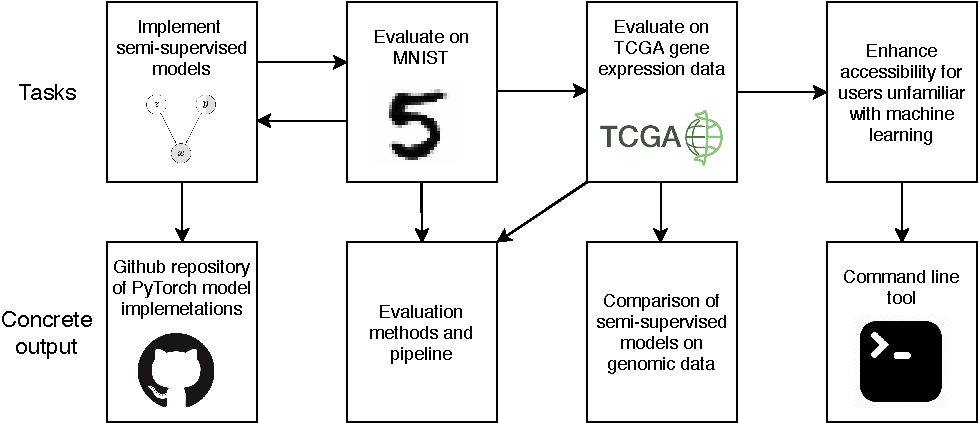
\includegraphics[scale=.9]{figs/workflow.pdf}
\caption{Project workflow}
\label{fig:workflow}
\end{figure}


\section{Related work}

Stacked denoising autoencoders have previously been used with gene expression data to derive the most informative
genes for distinguishing between healthy and cancerous cells~\cite{8217828}.

Likewise, variational autoencoders (Section~\ref{vae}) have been successfully used to extract a biologically relevant latent 
space from cancer transcriptomes ~\cite{Way2018ExtractingAB}. They and the semi-supervised variant (Section~\ref{ssVAE}) 
have also been used to model the change in the gene expression of tumours in response to certain drugs~\cite{10.1093/bioinformatics/btz158}.

Ladder networks have also been used in biologically relevant (non semi-supervised)
ways, achieving state-of-the-art accuracy in binary cancer classification~\cite{10.1007/978-3-319-78723-7_23}.

\chapter{Preparation}

\textit{A major part of this project involved reading and understanding the theory behind the models before implementing them. This theory
is described here and so there is overlap with the Implementation chapter, which contains more concrete details on model implementations. 
This chapter also contains information about the success 
criteria and resources used in the project.}

\section{Neural networks}

This project involves using \textbf{autoencoders} as a basis for semi-supervised learning. 
Autoencoder architectures are all based on \textbf{neural networks} so it is important to understand the basic principles.

\subsection{The perceptron}

The perceptron (or \textbf{artificial neuron}) is the basic element of the neural network. It takes in inputs $(x_1, ..., x_n)$ and 
multiplies these by \textbf{weights} $(w_1, ..., w_n)$, giving a linear combination of the inputs $x_1w_1 + ... + x_nw_n$, before applying 
an \textbf{activation function} $\sigma$~\cite{Art_Int}.

It is helpful to think of the inputs and weights as 
vectors $\vec{x}$ and $\vec{w}$, giving the combination as $\vec{x} \cdot \ \vec{w}$. A \textbf{bias} term $x_0=1$ may also be included and multiplied by 
weight $w_0$, giving $\vec{x} = [1, x_1, ..., x_n]$ and $\vec{w} = [w_0, w_1, ..., w_n]$. The bias can be thought of as the intercept
on a graph - if the neuron should have an output when all the inputs are zero it will be unable to model this correctly without a bias.

The function computed by the neuron is then:
\begin{equation}
  y = \sigma(\vec{x} \cdot \vec{w})
\end{equation}

The activation function applied will depend on what the neuron is being used for.
The main activation function used in this project is ReLU, which has the form:
\begin{align}
  \sigma(z) = max(0, z)
  \label{eq:relu}
\end{align}
It is used in the hidden layers of multilayer perceptrons to provide non-linearity, allowing the network to learn more 
complicated functions~\cite{relu}.

\subsection{Multilayer perceptrons}

Multilayer perceptrons consist of multiple perceptrons arranged into \textbf{layers}. 
Each neuron in a layer has its own set of weights
$\vec{w}$ and takes the ouputs of the previous layer (or the inputs to the network if the neuron is in the first layer) $\vec{x}$ in order to compute the 
output value $y$ for the neuron. This value is then used as an input to the next layer, or part of the output of the network if the neuron is in
the output layer.
\begin{figure}[H]
  \begin{center}
      \scalebox{.75}{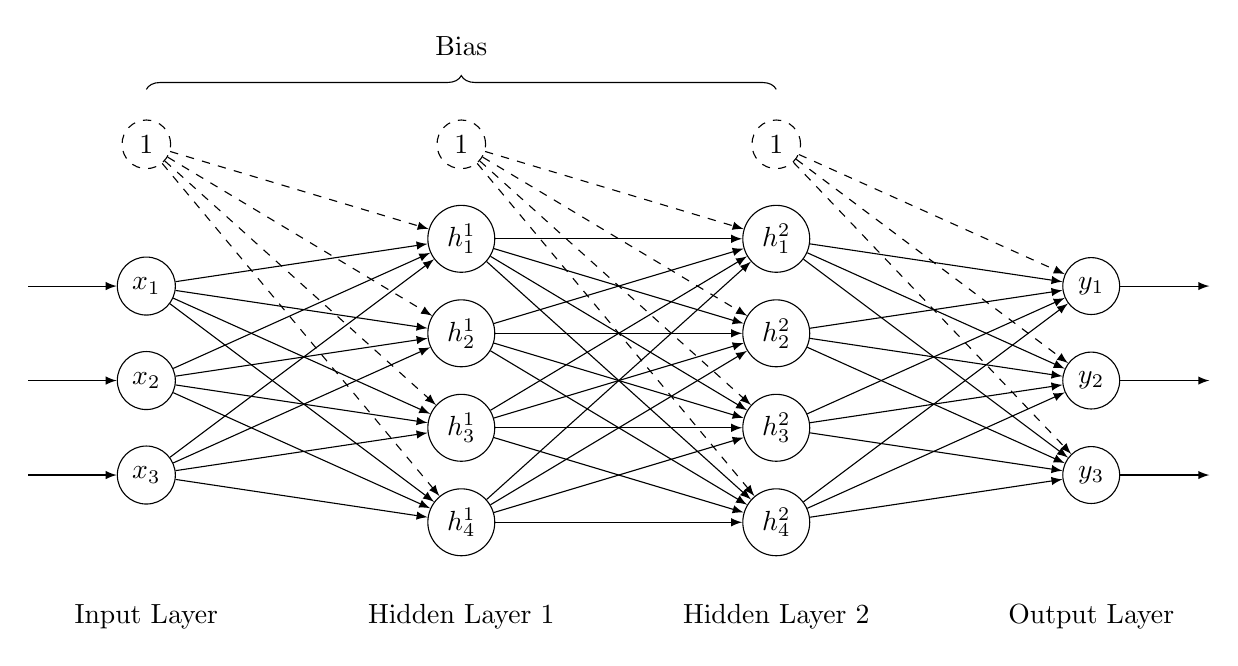
\begin{tikzpicture}
    \tikzstyle{place}=[circle, draw=black, minimum size = 4mm]
    
    % Input
    \draw node [dashed] at (0, 0) [place] (first_0) {$1$};
    \foreach \x in {1,...,3}
      \draw node at (0, -\x*1.2 - 0.6) [place] (first_\x) {$x_\x$};
    \foreach \x in {1,...,3}
      \draw [->] (-1.5, -\x*1.2 - 0.6) to (first_\x); 
    
    % Hidden 1
    \draw node [dashed] at (4, 0) [place] (second_0) {$1$};
    \foreach \x in {1,...,4}
      \node at (4, -\x*1.2) [place] (second_\x) {$h^{1}_\x$};

    % Hidden 2
    \draw node [dashed] at (8, 0) [place] (third_0) {$1$};
    \foreach \x in {1,...,4}
      \node at (8, -\x*1.2) [place] (third_\x) {$h^{2}_\x$};
    
    % Output
    \foreach \x in {1,...,3}
      \node at (12, -\x*1.2 - 0.6) [place] (fourth_\x) {$y_\x$};
    \foreach \x in {1,...,3}
      \draw [->] (fourth_\x) to (13.5, -\x*1.2 - 0.6); 

    \draw [decorate,decoration={brace,amplitude=5pt,raise=-2ex}]
      (0,1) -- (8,1) node[above,midway]{Bias};
      
    % Input -> Hidden 1
    \foreach \i in {1,...,4}
      \draw [->,dashed] (first_0) to (second_\i);
    \foreach \i in {1,...,3}
      \foreach \j in {1,...,4}
        \draw [->] (first_\i) to (second_\j);
    
    % Input -> Hidden 2
    \foreach \i in {1,...,4}
      \draw [->,dashed] (second_0) to (third_\i);
    \foreach \i in {1,...,4}
      \foreach \j in {1,...,4}
        \draw [->] (second_\i) to (third_\j);
    
    % Hidden -> Output
    \foreach \i in {1,...,3}
      \draw [->,dashed] (third_0) to (fourth_\i);
    \foreach \i in {1,...,4}
      \foreach \j in {1,...,3}
        \draw [->] (third_\i) to (fourth_\j);
    
    % Text
    \node at (0, -6) [black, ] {Input Layer};
    \node at (4, -6) [black, ] {Hidden Layer 1};
    \node at (8, -6) [black, ] {Hidden Layer 2};
    \node at (12, -6) [black, ] {Output Layer};
  \end{tikzpicture}}
      \caption{Illustration of a 4-layer multilayer perceptron}
      \label{fig:illustration_deep_network}
  \end{center}
\end{figure}
 
The reason for multi-layers neural networks is that they can model more \textbf{complex non-linear relationships}
~\cite{Goodfellow-et-al-2016} than single 
neurons and single-layer models are able to. Using non-linear activation functions such as ReLU \eqref{eq:relu} allow neurons to model simple 
non-linear functions, and combining these into layers allows them to model these more complex non-linear relationships.

I will denote the function computed by a neural network as $f_{\vec{\theta}}(\vec{x})$, where $\vec{\theta}$ denotes the
weights of the neural network.

\subsection{Neural networks for classification}

A dataset for classification training is given as pairs of numerical \textbf{features} and a \textbf{label}: $(\vec{x}, y)$. These features are 
the input to the network,
and the label is the target. Labels have to be transformed into a numerical representation to be used by the network.

\textbf{One-hot encoding} assigns an integer $i$ to each class and makes a vector of length $n$ (where $n$ is the 
number of classes), setting the $ith$ element to one and all other elements to zero. E.g., with three classes
the one-hot labels would be $[1, 0, 0]$ , $[0, 1, 0]$ and $[0, 0, 1]$. The network then has an output node corresponding to each class 
\cite{WhyOneHo55:online}.

The \textbf{softmax} function is then applied to the output of the network to give a probability distribution over the classes. It has the 
form below for each output node $i$, and ensures that the sum of all the output values is one.
\begin{align}
  \sigma(z)_{i} = \frac{e^{i}}{\sum_{k} e^{k}}
\end{align}
A single label can be returned by taking the index of the maximum value in the ouput and correlating that to the label index. 

The \textbf{loss} of the network is the difference between the output of the network and the correct label. The loss should be high 
when the network is performing poorly, and low when it is performing well. For classification the loss function used is the cross 
entropy loss, computed as:
\begin{align}
  J(\vec{\theta}) = - \vec{y} \cdot \log{f_{\vec{\theta}}(\vec{x})} \label{eq:ce}
\end{align}
This is high when the probability of the correct label is low, because $\lim_{x \to 0} -\log{x} = \infty$.

\subsection{Training the network} \label{train}

Neural networks have their weights randomly initialised, and training a neural network involves adjusting them 
($\vec{\theta}$) until the network reaches an acceptable loss or accuracy. This is done by computing 
the gradients of the weights with respect to the loss, and updating the parameters to move the loss towards 
a minimum.

\subsubsection{Updating the weights}

Forward propagation is the flow of information through the network from input features to output values. From these output values the loss is calculated. 
The weights of a neural network can then be updated by first finding the gradient of the loss with respect to these weights.
The process of computing these gradients is called \textbf{backpropagation} and a full derivation can be found in Appendix~\ref{backprop}. The important notation is:

\begin{itemize}
  \item $\theta$ is a vector of all the weights in the network
  \item $J(\vec{\theta})_k$ is the loss for the $kth$ sample in the training set
  \item $\nabla_{\vec{\theta}} J(\vec{\theta})_k$ is a vector of gradients of the loss with respect to all the weights 
\end{itemize}

Once the gradients have been calculated the weights are updated. By moving the weights incrementally in the direction of steepest 
negative gradient the loss should decrease as the parameters are shifting it towards a minimum. The model thus gets
better at modelling the training set. These incremental steps are called \textbf{gradient descent}. The weight update rule is: 
\begin{align}
  \vec{\theta} & := \mathbf{\vec{\theta}} - \eta \sum_{k} \frac{\partial J(\vec{\theta})_k}{\partial \mathbf{\vec{\theta}}} \\
  & := \mathbf{\vec{\theta}} - \eta \sum_{k} \nabla_{\vec{\theta}} J(\vec{\theta})_k \\
  & := \mathbf{\vec{\theta}} - \eta \nabla_{\vec{\theta}} \sum_{k} J(\vec{\theta})_k \label{eq:weight}
\end{align}

$\eta$ is a \textbf{hyperparameter}. Hyperparameters are parameters of the model that are not trained but are set by the user before training.
$\eta$ is called the \textbf{learning rate} and controls the size of the step taken each time the weight is updated. If the learning rate is 
too high the weights can ``jump'' over minima, and even diverge out of a minimum, but if the rate is too low it can take too long to converge,
or get stuck in a less desirable local minima. The step size is proportional to the magnitude of the gradient, allowing the optimizer to 
take a larger step towards a minimum if the gradient is steeper.

\subsubsection{Batch learning} \label{batch}

A neural network is generally run over a fixed number of samples for each iteration. This is called 
mini-batch gradient descent and it is the most popular because it has stability advantages over stochastic gradient descent (one sample at a time),
and computational advantages over batch (the entire dataset every iteration). 
Stochastic gradient descent has more noise as each update is based on an individual example, causing the weights to jump around more. It also doesn't take advantage of the 
parallelisation possiblity of GPUs - it's much more efficient to send multiple samples through at once. Batch has the problem of storing the whole 
dataset in memory, and only making one update per pass through the dataset can mean the model takes longer to converge to the best parameters. Mini-batch manages to
have less noise than stochastic due to averaging over multiple samples, while also taking advantage of parallelisation and not requiring huge amounts of memory.

\subsubsection{Summary}

One complete pass through the dataset 
is called an \textbf{epoch} and 
training involves running forward and backpropagation for a certain number of epochs to minimise the loss
on the training set and cause the model to converge to a good approximation to the real function. The pseudocode for training the network 
is shown below.
\begin{algorithm}
  \begin{algorithmic}[1]
    \Procedure{Training}{$i$, $\mathcal{D}$, $\eta$, \texttt{model}, \texttt{loss\char`_function}}
    \For{$i$ epochs}
    \For{mini-batch $\mathcal{M}$ in $\mathcal{D}$}
    \State \texttt{data, labels} = $\mathcal{M}$
    \State \texttt{out} = \texttt{model(data)}
    \State $\mathcal{J}$ = \texttt{loss\char`_function(out, labels)}
    \State \texttt{model}.$\vec{\theta}$ = \texttt{model}.$\vec{\theta}$ - $\eta \nabla_{\vec{\theta}} \mathcal{J}$ 
    \EndFor
    \EndFor
    \EndProcedure
  \end{algorithmic}
  \caption{Train neural network via mini-batch gradient descent} 
  \label{alg:train}
\end{algorithm}

\section{The manifold hypothesis}

\textbf{Dimensionality} refers to the number of features needed to specify data. For example, a very popular machine learning dataset
is MNIST, containing 28x28 grayscale images of handwritten digits. The dimensionality of each datapoint is 784, as that is the
number of pixels specifying each image.

\textbf{The manifold hypothesis} suggests that high-dimensional data can actually be viewed as lying on or near to a
lower-dimensional manifold embedded in this higher-dimensional space.

The definition of an n-dimensional manifold is ``a 
topological space that is locally Euclidean'', i.e. there is a neighbourhood around each point on the manifold that can be describe as n-dimensional 
Euclidean space. It is much easier to grasp with an intuitive example - imagine that all the datapoints in a 
dataset lie on piece of paper, and so can be described with two features, an $x$ and $y$ axis. If the paper is scrunched up 
it now has a three dimensional shape, but the data still lies on a two-dimensional manifold. Unscrunch the paper and it can still 
be described with only two features.
\begin{figure}[H]
  \centering
  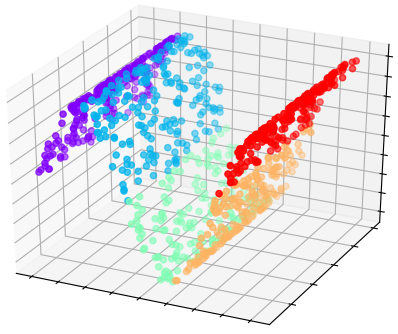
\includegraphics[scale=.75]{figs/manifold.png}
  \caption{Points on a 2-dimensional manifold embedded in 3-dimensional space}
  \label{fig:manifold}
\end{figure}

The manifold hypothesis suggests that many features in high-dimensional data are actually redundant,
i.e. it can be described using fewer features. Again this can be seen intuitively in that the set of 784 pixel images 
that look like a recognisable digit is a very small subset of 784 pixel images - randomly selected pixel values look like 
random noise, suggesting that there is a lot of redundancy in the MNIST features.
\begin{figure}[H]
  \centering
  \begin{subfigure}[b]{0.4\linewidth}
    \centering
    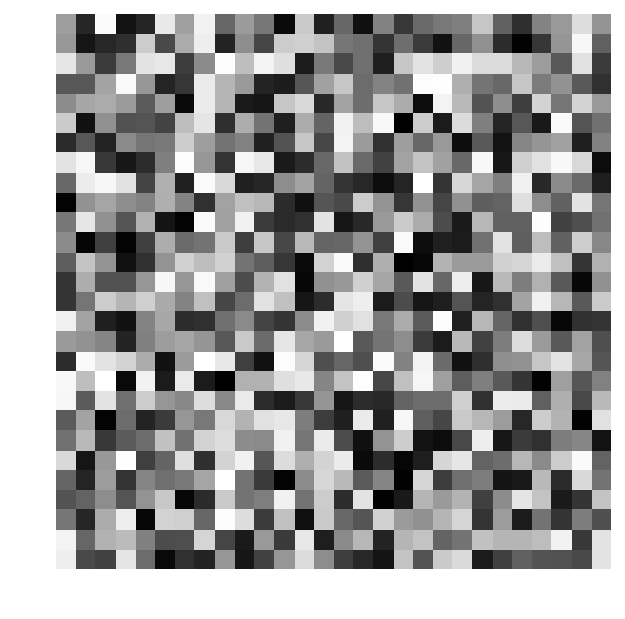
\includegraphics[scale=.25]{figs/rand_noise.pdf}
    \caption{Pixel values selected randomly}
  \end{subfigure}
  \begin{subfigure}[b]{0.4\linewidth}
    \centering
    
\includegraphics[scale=.25]{figs/digit.pdf}
    \caption{MNIST digit}
  \end{subfigure}
  \caption{Demonstrating redundancy of features in MNIST dataset}
  \label{fig:digit}
\end{figure}

This leads to \textbf{non-linear dimensionality-reduction} techniques. By finding this lower-dimensional
manifold the data can be explained with fewer features and possibly be more easily separated and classified. Going back to the paper example,
linear-dimensionality reduction techniques would be able to find the 2D embedding if the paper were 
rotated, translated or stretched, but would be unable to unscrunch the paper, as that is a non-linear transformation. Autoencoders are 
used for non-linear dimensionality reduction, and are described in the next section.

\section{Autoencoders}

Autoencoders use neural networks in an unsupervised way to learn new \textbf{latent} representations of data, typically with reduced 
dimensionality (i.e. there are fewer features in the latent data than in the input data). The use of neural networks allow the autoencoder 
to learn a non-linear mapping from the data to the latent representation.

Autoencoders compromise an encoder and a decoder. The encoder takes in the original data, $\vec{x}$, 
and outputs a latent representation, $\vec{z} = f_{\vec{\theta}}(\vec{x})$. The decoder then takes this latent representation and 
attempts to reconstruct $\vec{x}$, outputting $\vec{\hat{x}} = h_{\vec{\phi}}(\vec{z})$. This allows an unsupervised problem to be turned 
into a supervised problem, using $\vec{x}$ as the target.
\begin{figure}[H]
  \begin{center}
      \scalebox{.75}{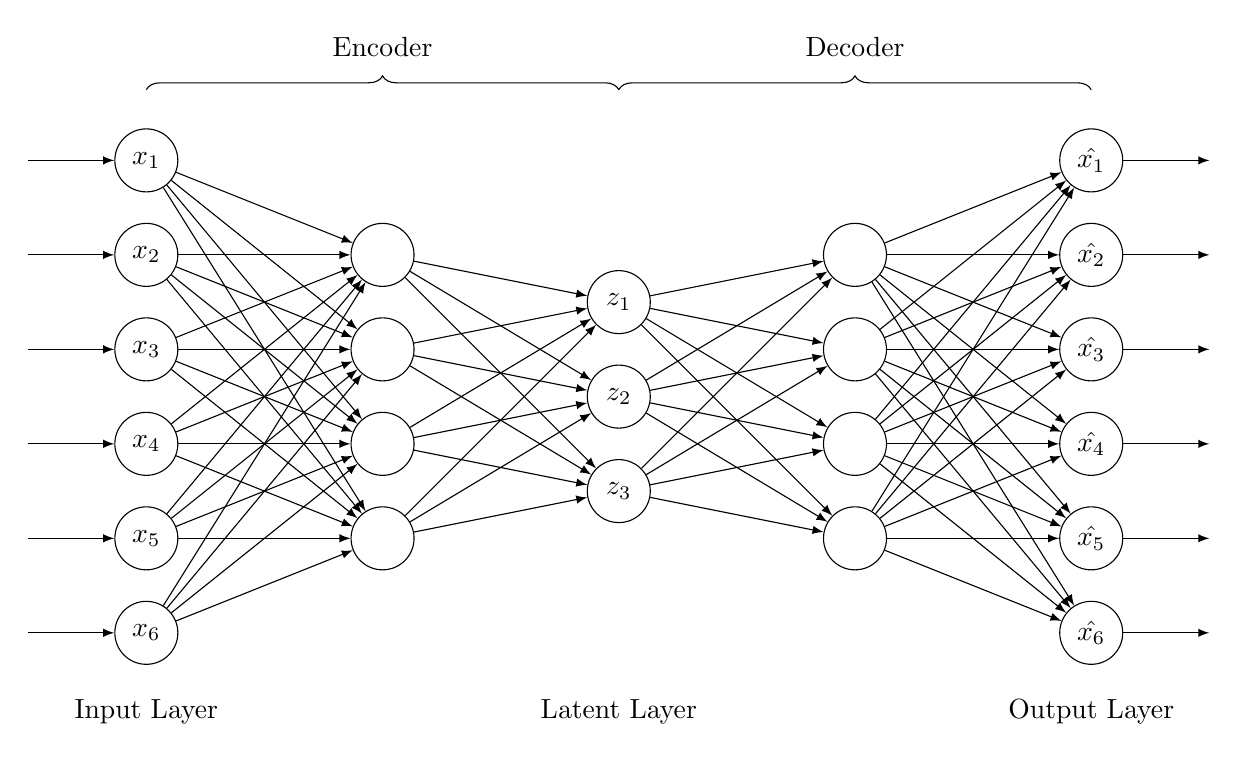
\begin{tikzpicture}
    \tikzstyle{place}=[circle, draw=black, minimum size = 8mm]

    % Input
    \foreach \x in {1,...,6}
        \draw node at (0, -\x*1.2) [place] (first_\x) {$x_\x$};

    % Hidden 1
    \foreach \x in {1,...,4}
        \node at (3, -1.2 -\x*1.2) [place] (second_\x){};

    % Latent
    \foreach \x in {1,...,3}
        \node at (6, -1.8 -\x*1.2) [place] (third_\x){$z_\x$};

    % Hidden 2
    \foreach \x in {1,...,4}
        \node at (9, -1.2 -\x*1.2) [place] (fourth_\x){};

    % Output
    \foreach \x in {1,...,6}
        \draw node at (12, -\x*1.2) [place] (fifth_\x) {$\hat{x_\x}$};
        
    \foreach \i in {1,...,6}
        \draw [->] (-1.5, -\i*1.2) to (first_\i);

    \foreach \i in {1,...,6}
        \foreach \j in {1,...,4}
        \draw [->] (first_\i) to (second_\j);

    \foreach \i in {1,...,4}
        \foreach \j in {1,...,3}
            \draw [->] (second_\i) to (third_\j);

    \foreach \i in {1,...,3}
        \foreach \j in {1,...,4}
        \draw [->] (third_\i) to (fourth_\j);

    \foreach \i in {1,...,4}
        \foreach \j in {1,...,6}
            \draw [->] (fourth_\i) to (fifth_\j);

    \foreach \i in {1,...,6}
        \draw [->] (fifth_\i) to (13.5, -\i*1.2);

    \draw [decorate,decoration={brace,amplitude=5pt,raise=-2ex}]
        (0,0) -- (6,0) node[above,midway]{Encoder};
    \draw [decorate,decoration={brace,amplitude=5pt,raise=-2ex}]
        (6,0) -- (12,0) node[above,midway]{Decoder};

    % Text
    \node at (0, -8.2) [black, ] {Input Layer};
    \node at (6, -8.2) [black, ] {Latent Layer};
    \node at (12, -8.2) [black, ] {Output Layer};
\end{tikzpicture}}
      \caption{Illustration of a simple autoencoder}
      \label{fig:illustration_autoencoder}
  \end{center}
\end{figure}

\subsection{Simple autoencoders}

Simple autoencoders constrain the network by making the number of latent features smaller than the number of input
features. This prevents the network from simply learning the identity function, and hopefully results in an informative latent space.

\subsubsection{Training}
Autoencoders can be trained end to end using backpropagation as explained in Section \ref{train}. The target $\vec{x}$ and output 
$\vec{\hat{x}}$ are both vectors and so 
the \textbf{squared Euclidean distance}\footnote{also known as mean square error} is used as the loss per datapoint. Both the encoder weights 
$\vec{\theta}$ and 
decoder weights $\vec{\phi}$ 
are trained at the 
same time; the gradients are backpropagated through the decoder to the latent layer and then back through the encoder. 

\subsection{Denoising autoencoders}

Denoising autoencoders corrupt the input data with noise (e.g. by adding Gaussian noise) giving $\tilde{\vec{x}}$, which is then used as the 
input to the network. However, the target is the uncorrupted input data, 
$\vec{x}$. The aim is to force the autoencoder to learn a better set of features because it not only has to reconstruct the data but also 
has to remove the noise. They can be trained in the same way as a simple autoencoder.

\subsection{Variational autoencoders} \label{vae}

Variational autoencoders were 
introduced by Kingma and Welling in 2013~\cite{DBLP:journals/corr/KingmaW13} and have become one of the most popular unsupervised learning techniques. 
They are based on Bayesian inference, and differ from other autoencoders in that the encoder outputs
the parameters of a probability distribution over the latent variables, rather than a single configuration.
\begin{figure}[H]
  \begin{center}
      \scalebox{.75}{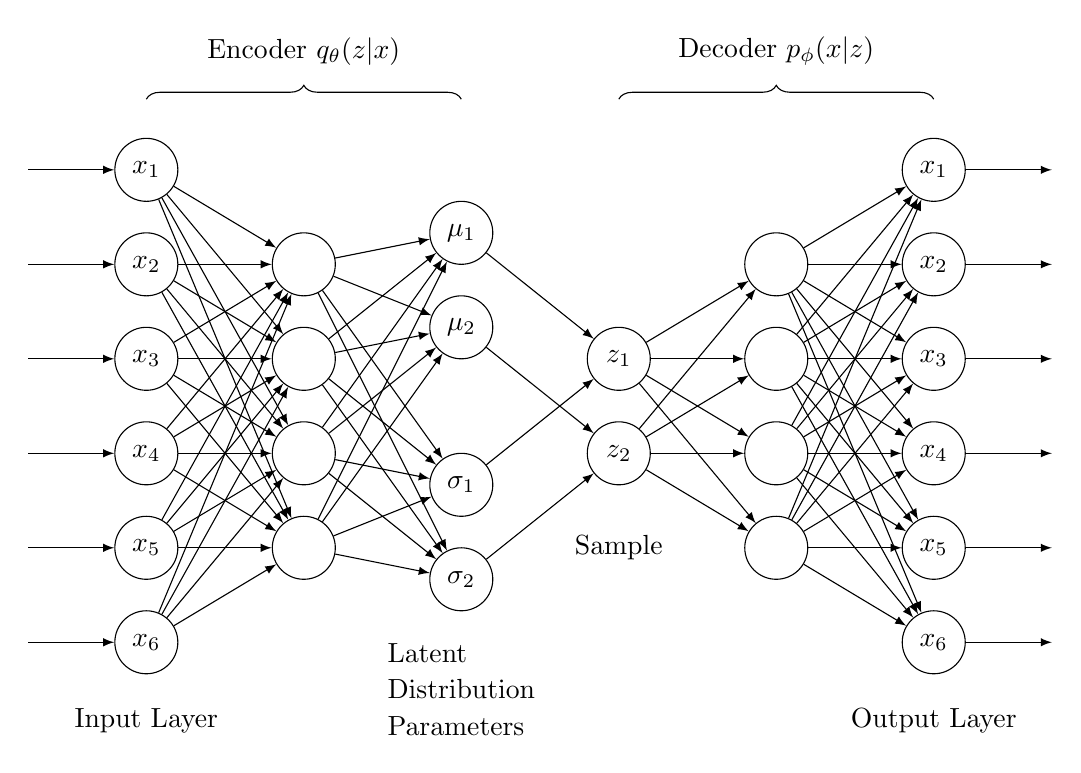
\begin{tikzpicture}
    \tikzstyle{place}=[circle, draw=black, minimum size = 8mm]
    
    % Input
    \foreach \x in {1,...,6}
        \draw node at (0, -\x*1.2) [place] (first_\x) {$x_\x$};
    
    % Hidden 1
    \foreach \x in {1,...,4}
        \node at (2, -1.2 -\x*1.2) [place] (second_\x){};

    % Mu
    \foreach \x in {1,...,2}
        \node at (4, -0.8 -\x*1.2) [place] (mu_\x){$\mu_\x$};

    \foreach \x in {1,...,2}
        \node at (4, -4 -\x*1.2) [place] (logvar_\x){$\sigma_\x$};

    \foreach \x in {1,...,2}
        \draw node at (6, -2.4 -\x*1.2) [place] (sample_\x){$z_\x$};

    % Hidden 2
    \foreach \x in {1,...,4}
        \node at (8, -1.2 -\x*1.2) [place] (fourth_\x){};
    
    % Output
    \foreach \x in {1,...,6}
        \draw node at (10, -\x*1.2) [place] (fifth_\x) {$x_\x$};
        
    \foreach \i in {1,...,6}
        \draw [->] (-1.5, -\i*1.2) to (first_\i);

    \foreach \i in {1,...,6}
        \foreach \j in {1,...,4}
        \draw [->] (first_\i) to (second_\j);

    \foreach \i in {1,...,4}
        \foreach \j in {1,...,2}
            \draw [->] (second_\i) to (mu_\j);
    \foreach \i in {1,...,4}
        \foreach \j in {1,...,2}
        \draw [->] (second_\i) to (logvar_\j);

    \foreach \i in {1,...,2}
        \draw [->] (logvar_\i) to (sample_\i);
    
    \foreach \i in {1,...,2}
        \draw [->] (mu_\i) to (sample_\i);

    \foreach \i in {1,...,2}
        \foreach \j in {1,...,4}
        \draw [->] (sample_\i) to (fourth_\j);
    
    \foreach \i in {1,...,4}
        \foreach \j in {1,...,6}
        \draw [->] (fourth_\i) to (fifth_\j);

    \foreach \i in {1,...,6}
        \draw [->] (fifth_\i) to (11.5, -\i*1.2);

    \draw [decorate,decoration={brace,amplitude=5pt,raise=-2ex}]
        (0,0) -- (4,0) node[above,midway]{Encoder $q_\theta(z|x)$};
    \draw [decorate,decoration={brace,amplitude=5pt,raise=-2ex}]
        (6,0) -- (10,0) node[above,midway]{Decoder $p_\phi(x|z)$};
    
    % Text
    \node at (0, -8.2) [black, ] {Input Layer};
    \node at (4, -7.8) [black, align=left] {Latent \\ Distribution\\ Parameters};
    \node at (6, -6) [black, ] {Sample};
    \node at (10, -8.2) [black, ] {Output Layer};
\end{tikzpicture}}
      \caption{Illustration of a Gaussian variational autoencoder}
      \label{fig:gauss_vae}
  \end{center}
\end{figure}

The central idea of variational autoencoders is that the data $\vec{x}$ has been generated from some lower-dimensional latent
representation $\vec{z}$. The latent distribution describes the variation in the data, and so these are called 
\textbf{latent variable models}. Each datapoint $\vec{x_{i}}$ is generated by:
\begin{itemize}
  \item sampling $\vec{z_{i}}$ from the prior distribution over $\vec{z}$: $\vec{z_{i}} \sim p(\vec{z})$, 
  \item sampling $\vec{x_{i}}$ from the conditional distribution $p(\vec{x}|\vec{z})$ (known as the likelihood): \\ 
  $\vec{x_{i}} \sim p(\vec{x}|\vec{z}=\vec{z_{i}})$
\end{itemize}

The prior $p(\vec{z})$ can be thought of as constraining the possible space of latent variables. In an unconstrained latent space, a
normal autoencoder could place the same character written in different styles in different areas of n-dimensional Euclidean space (where n is the 
dimensionality of $z$) as the latent representation is a vector of unconstrained real numbers. This is detrimental to learning a meaningful 
latent space, and by constraining this space with a prior it should force the model to keep the representations of similar datapoints close~\cite{Tutorial70:online}.

The decoder of the VAE is a neural network that models the likelihood, represented as $p_{\vec{\phi}}(\vec{x}|\vec{z})$. Once the VAE is 
trained, new samples similar to 
those in the training set can be generated by sampling from the prior and passing this into the decoder; this is why VAEs are often
referred to as generative models.

In most situations where unsupervised learning is useful, only $\vec{x}$ is known. The goal is then to infer $\vec{z}$.
Inference in the model refers to finding good values of the latent variables given the data. This can be done by computing the
posterior, $p(\vec{z}|\vec{x})$. Using Bayes' rule we have:
\begin{equation}
  p(z|x) = \frac{p(x|z)p(z)}{p(x)}
\end{equation}

The denominator $p(\vec{x})$ is known as the evidence, and calculating it is intractable as it has to be computed by marginalizing out $\vec{z}$:
\begin{equation}
  p(x) = \int p(x|z)p(z) dz
\end{equation}

Computing this integral requires exponential time as it has to be computed over all the possible configurations of
the latent variables. Therefore the posterior is approximated using a neural network $q_{\vec{\theta}}(\vec{z}|\vec{x})$. 
This is the encoder.

\subsubsection{Training}

The loss function used for a variational autoencoder can be derived by maximizing the probability of the evidence.
This makes sense intuitively, as a good model should maximise the probability of the real data~\cite{SVIPartI90:online}. A full derivation
of this loss can be found in Appendix~\ref{vae_loss}, but the final form is below:
\begingroup
\allowdisplaybreaks
\begin{align}
  \log p(x) = \mathbb{E}_q [\log p(x|z)] - D_{KL}(q(z|x)||p(z))
\end{align}
\endgroup

This is the \textbf{evidence lower bound} (ELBO). Maximizing the ELBO maximizes the probability of the 
evidence in the model, meaning the model fits the data as well as possible. The two terms in the ELBO correspond to the negative 
reconstruction loss (squared Euclidean distance) between the input and output, and the \textbf{Kullback-Leibler divergence} (KLD) between 
the computed posterior and the prior distribution of the latent variables. 
The KLD measures the difference between two probability distributions, and this acts as a regularizing term, constraining the distribution 
of the latent variables to be close to the prior. Taking the 
negative of the ELBO gives the loss function for the variational autoencoder. Minimizing this loss function is equivalent to maximising the ELBO.

\paragraph{The Gaussian VAE}is the most common and the one used in this project. The prior $p(\vec{z})$ is chosen to be the standard Gaussian, 
$\mathcal{N}(0, 1)$,
for every latent variable. The output from the encoder is a vector of means $\vec{\mu}$ and standard deviations $\vec{\sigma}$ of normal distributions. 
During training, data is fed in mini-batches into the encoder and latent variables are then sampled from the encoder output: 
$\vec{z_{i}} \sim \mathcal{N}(\vec{\mu}, \vec{\sigma}^{2})$. These are fed into the decoder which outputs a reconstruction $\vec{\hat{x}}$. 
The loss for each datapoint is then computed as the reconstruction loss between $\vec{\hat{x}}$ and $\vec{x}$ and the KLD between
$\mathcal{N}(\vec{\mu}, \vec{\sigma}^{2})$ and $\mathcal{N}(0, 1)$.

Training is done by backpropagation but
it is not possible to backpropagate the reconstruction loss through the drawing of the random sample, and so 
\textbf{the reparameterization trick} is used. 
An explanation can be found in Appendix ~\ref{reparam}.

\section{Semi-supervised models} \label{ss_models}

Semi-supervised learning involves leveraging unlabelled data to increase model performance on supervised learning tasks. 
In most fields, unlabelled data is much easier to obtain than labelled data. I noted in the Introduction that wealth of gene 
expression data for many different organisms is available online, albeit that the phenotype a researcher wants 
to study is often not included. With standard supervised learning this data is unusable, but semi-supervised learning
can use it to improve performance. 

\subsection{Dimensionality reduction (M1)} \label{m1}

The simplest semi-supervised model in this project relies on the manifold hypothesis. It uses a variational autoencoder to construct a
reduced dimensionality representation of the data that should cluster similar samples together, and is partially based 
on the Kingma M1 model~\cite{DBLP:journals/corr/KingmaRMW14}. The idea is that it should be 
easier to classify the datapoints in this latent dimension, even with a limited amount of labelled data.

\subsection{Network pre-training} \label{sdae}

\textbf{Stacked denoising autoencoders} are a way of pre-training deep networks one layer at a time, using unlabelled data. 
Each hidden layer in the network is 
trained as part of a one-layer denoising autoencoder, with the layer to be trained used as the encoder and a new temporary layer constructed
as the decoder. The autoencoder takes the ouput from the previous layer in the network and uses this as the input, injecting noise before 
passing it through the autoencoder and attempting to reconstruct the clean input. The reconstruction loss is then backpropagated through 
the autoencoder only (no other layers of the deep network) and the weights are updated. The loss computed by the autoencoder is referred to 
as an unsupervised ``local denoising criterion''~\cite{Vincent:2010:SDA:1756006.1953039} as it does not require a label and is computed only 
for one layer at a time rather than the whole network.

The network is trained one layer at a time, beginning with the first hidden layer. Once the reconstruction loss for the denoising autoencoder has 
converged for the layer, the decoder is discarded, and the next layer is trained in the same way, using the output of the previously trained
layer as input.

Once this unsupervised pre-training is finished the model is then \textit{fine-tuned} by running normal supervised training, backpropagating
classification loss through the entire network and updating the weights.

Unsupervised pre-training with a stacked denoising autoencoder provides a good prior to the supervised training.
The pre-training procedure provides an initialization point for the supervised training where the parameters are restricted, hopefully to an area 
closer to the global minimum for the loss function~\cite{Erhan:2010:WUP:1756006.1756025}.

\subsection{The semi-supervised VAE (M2)} \label{ssVAE}

The semi-supervised VAE is a model introduced by Kingma et al.~\cite{DBLP:journals/corr/KingmaRMW14} that extends the VAE to include label information. 
The assumption used is that the data $\vec{x}$ is generated from both a discrete label $y$ and a continuous latent representation 
$\vec{z}$, which are marginally independent of each other.
Therefore $y$ encodes the class of the data, while $\vec{z}$ encodes everything else. In the MNIST dataset this means that $y$ encodes
what digit the character is, while $\vec{z}$ encodes the style. The generative model (the decoder) works by sampling $y$ from a 
categorical distribution $p(y)$ and by sampling $\vec{z}$ from a continuous distribution $p(\vec{z})$ (usually a Gaussian), before computing 
$p(\vec{x}|y, \vec{z})$ using a neural network $p_{\vec{\phi}}(\vec{x}|y, \vec{z})$.
\begin{figure}[H]
  \begin{subfigure}[b]{0.5\textwidth}
    \centering
    \scalebox{.9}{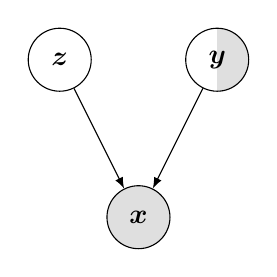
\begin{tikzpicture}
    \draw node at (0, 0) [place] (z) {$\vec{z}$};
    \draw node at (2, 0) [place] (y) {$\vec{y}$};
    \draw node at (1, -2) [place] (x) {$\vec{x}$};

    \begin{scope}[on background layer]
    \fill[fill=gray!25] (x.0) arc [start angle=0, end angle=360, radius=4mm];
    \fill[fill=gray!25] (y.270) arc [start angle=270, end angle=450, radius=4mm];
    \end{scope}

    \draw [->] (z) to (x);
    \draw [->] (y) to (x);
\end{tikzpicture}}
    \caption{The generative model}
  \end{subfigure}
  \begin{subfigure}[b]{0.5\textwidth}
    \centering
    \scalebox{.9}{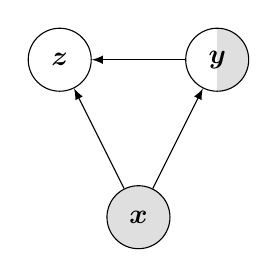
\begin{tikzpicture}
    \draw node at (0, 0) [place] (z) {$\vec{z}$};
    \draw node at (2, 0) [place] (y) {$\vec{y}$};
    \draw node at (1, -2) [place] (x) {$\vec{x}$};

    \begin{scope}[on background layer]
    \fill[fill=gray!25] (x.0) arc [start angle=0, end angle=360, radius=4mm];
    \fill[fill=gray!25] (y.270) arc [start angle=270, end angle=450, radius=4mm];
    \end{scope}

    \draw [->] (x) to (y);
    \draw [->] (x) to (z);
    \draw [->] (y) to (z);
\end{tikzpicture}}
    \caption{The inference model}
  \end{subfigure}
  \caption[Semi-supervised VAE]{The semi-supervised VAE \\ (shading indicates that a variable in the dataset is observed)}
  \label{fig:ss_vae}
\end{figure}

In the semi-supervised model there are two inference cases. When the data is labelled the question is how to infer $\vec{z}$ from $\vec{x}$ and $y$.
Both $\vec{x}$ and $\vec{y}$ are used as input to the encoder, while $y$ and $\vec{z}$ are used as input to the decoder.
This helps the encoder to learn to separate the representation of $y$ and $\vec{z}$, so that $\vec{z}$ contains
no information about the label. The semi-supervised VAE in this project uses a Gaussian distribution as the prior distribution for 
$\vec{z}$ (like the unsupervised VAE), and the encoder models $q(\vec{z}|\vec{x}, y)$ with a network $q_{\theta}(\vec{z}|\vec{x}, y)$. For labelled data 
the model should 
maximise the evidence $p(\vec{x}, y)$, the probability of the real labelled data. This leads to a variant of the ELBO by marginalizing
out $z$:
\begin{align}
  \log p(x, y) & = \mathbb{E}_q [\log p(x|y, z) + \log p(y)] - D_{KL}(q(z|x, y)||p(z)) \\
  & = -\mathcal{L}(x, y)
\end{align}

The derivation is not included in the Kingma paper~\cite{DBLP:journals/corr/KingmaRMW14}, which includes only the line above and so I had 
to derive it myself. The derivation can be found in Appendix~\ref{ssvae_loss}.

It is very similar to the ELBO for the normal VAE, except that there is now a prior over $y$. This encodes previous knowledge about the 
distribution of the classes $y$, penalizing the model more when the label is of a low probability class. This is unimportant for the labelled
data as the previous knowledge is drawn from this data, but becomes important for the unlabelled data, and the connection between the two can be 
seen in the unlabelled ELBO below. A good model maximises the ELBO and therefore minimises $\mathcal{L}(x, y)$, which is used as the loss function.

When the data is unlabelled, the problem is of inferring both $y$ and $\vec{z}$ from $\vec{x}$, $q(y, \vec{z}|\vec{x})$. The evidence in the unlabelled 
case is $p(\vec{x})$,
and the ELBO can be derived by marginalizing out both $y$ and $\vec{z}$:
\begin{align}
  \log p(x) & = \sum_{y} q(y|x)(-\mathcal{L}(x, y)) + \mathcal{H}(q(y|x)) \\
  & = -\mathcal{U}(x, y)
\end{align}
This derivation is also in Appendix~\ref{ssvae_loss}.

The marginalization of $y$ is done by summation because the labels are discrete. Looking at the penultimate line of the derivation there is
the term $q(y|x)$. This is classification, inferring $y$ from $\vec{x}$. This classifier is parameterised
by a neural network, and outputs a categorical distribution over the labels.

The summation term is referred to as ``classification as inference'' by Kingma~\cite{DBLP:journals/corr/KingmaRMW14}. For each label the labelled loss with 
respect to the data and that label is calculated and then multiplied by the probability of the label. This means that if a particular label
leads to a bad reconstruction (implying that the label was incorrect) and the classifier assigns a high probability to that label, 
the loss to the classifier will be very high, and minimizing this loss should lead to better classification. The prior over $y$ in $\mathcal{L}(x, y)$
becomes important here as it discourages the classifier from assigning a high probability to an unlikely class. All of this means that 
the classifier can learn directly from unlabelled data, with the small amount of labelled data providing a guide to good reconstructions.

The pipelines for labelled and unlabelled data are slightly different. Labelled data is fed directly into the encoder
along with its label, and the loss function $\mathcal{L}(x, y)$ is calculated and backpropagated through the network. Unlabelled data is 
first put through the classifier, before it is fed into the encoder once with each label allowing $\mathcal{U}(x)$ to be computed and 
backpropagated through the network.

Currently at no point does the classifier learn directly from the labelled data, inhibiting the model. To remedy
this the labelled loss function is modified to include an extra term, the cross entropy loss~\eqref{eq:ce} between the real label and the 
label the classifier outputs for the data. This modified version is then:
\begin{align}
  \mathcal{J}(x, y) = \mathcal{L}(x, y) - \alpha (y \cdot \log q(y|x))
\end{align}

$\alpha$ is a hyperparameter that controls the weighting of the supervised loss, and is configured depending on the amount of labelled and 
unlabelled data available.

The model can now learn to classify from both labelled and unlabelled data at the same time, and so does not require pretraining as
the previous models did.

\subsection{The ladder network} \label{ladder}

The ladder network is the most recent of the models included in this project, having first been described by Valpola in 2014
~\cite{DBLP:journals/corr/Valpola14}, and then expanded upon in 2015~\cite{DBLP:journals/corr/RasmusVHBR15}. 
It has some similarity to the SDAE, using an unsupervised local denoising criterion, but the structure of the model is very different.
The model is made up of an encoder and decoder, like an autoencoder, but with lateral connections between the layers in the encoder 
and decoder. The final classifier is the encoder.

\begin{figure}[H]
  \centering
  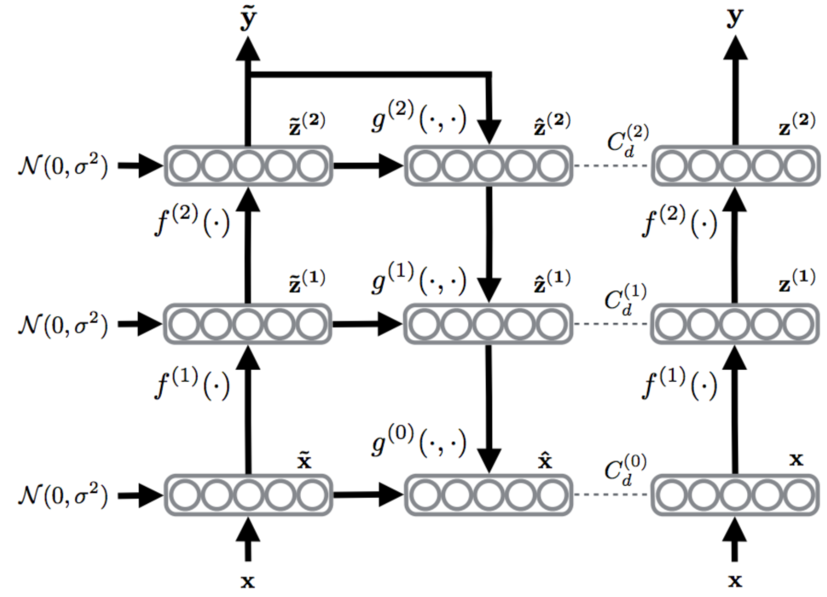
\includegraphics[scale=0.4]{figs/ladder.png}
  \caption[Illustration of the ladder network]{Illustration of the ladder network \\ (Source: Rasmus et al.~\cite{DBLP:journals/corr/RasmusVHBR15})}
  \label{fig:ladder}
\end{figure}

The ladder network is a hierarchical latent variable model, which differ from the latent variable models
looked at so far in that it attempts to represent the data using multiple layers of latent variables, rather than a 
single layer. 
In the normal autoencoder or VAE the single latent layer $\vec{z}$ has to encode everything about the data $\vec{x}$, otherwise the reconstruction it generates 
will be very poor. With a hierarchical model each layer models only some information about $\vec{x}$, with the higher layers able to be 
more abstract, 
as they don't have to model the details encoded in the lower layers. 

For example, using MNIST, $\vec{z}$ in an
autoencoder cannot just be the digit label as this does not provide enough information to reconstruct the original image well. 
In a hierarchical latent variable model the highest
level latent variable is able to be very abstract and only encode the label, as the other layers in the model provide less abstract 
information (e.g about style and location) that can lead to a good reconstruction.

The reason this works in the ladder network is because the lateral connections``leak'' information from layers in the encoder to the decoder. 
This means that each decoder layer
receives information both from the previous decoder layer and the corresponding encoder layer. The encoder layer passes some information which
the subsequent encoder layers then no longer have to model, as the decoder will receive it directly from the encoder layer.

This structure, with the representation becoming more abstract in higher level layers, is also analagous to how supervised learning works, with the layers 
further into the network modelling more complicated and abstract features, and with the final layer just outputting a class label.

The way these lateral connections work is that
at the input to each decoder layer $\vec{u}^{(l)}$ the corresponding encoder representation $\vec{z}^{(l)}$ and the output of the previous decoder layer $\vec{u}^{(l+1)}$ are combined
using a combinator function $g$. $g$ has trainable parameters (weights), but this leads to a problem where the lowest possible unsupervised loss can be 
achieved by $g$ in the first layer learning to copy $\vec{z}^{(0)}$ and completely ignoring $\vec{u}^{(l+1)}$, which corresponds to copying the input directly to the output at the bottom layer.
This short circuits the autoencoder, and in order to prevent this, Gaussian noise (sampled from $\mathcal{N}(0, 1)$) is added to the input to each layer 
in the encoder. Each encoder layer then has the representation $\vec{\tilde{z}}^{(l)}$ and this noise means that just copying over the input no longer minimises the loss function. 

However, if the unsupervised loss function used is simply the reconstruction loss between the decoder output $\vec{\hat{x}}$ and the encoder input $\vec{x}$, the first layer of 
the network still has a disproportionate
influence on the loss. In order to remedy this Valpola proposes adding a local denoising criterion. This involves adding a cost function at each layer of the decoder,
namely the reconstruction loss between $g(\vec{\tilde{z}}^{(l)}, \vec{u}^{(l+1)})$ (which is $\vec{\hat{z}}^{(l)}$, a denoised representation of $\vec{\tilde{z}}^{(l)}$) and $\vec{z}^{(l)}$, the clean 
representation from layer $l$ of the encoder. In order to generate both the clean and noisy encoder representations, the encoder is run twice per training iteration,
once without the added noise to generate $\vec{z}^{(l)}$, and once with noise to generate $\vec{\tilde{z}}^{(l)}$. These local cost functions require all the layers to learn in order
to make a meaningful representation that can be denoised well. Each layer loss is multiplied by a hyperparameter $\lambda_{l}$ according to how important the denoising cost
of the layer is, before being summed together to give a final unsupervised cost function per sample of:

\begin{align}
  \mathcal{U}(x) = \sum_{l} |z^{(l)} - \hat{z}^{(l)}|^{2}
\end{align}

The model as explained so far allows the ladder network to learn abstract features in the higher layers. However, without supervised data and a supervised loss function the 
features learned are unlikely to be useful for the classification task. The small amount of labelled data is used as a guide for this. The classifier 
is the encoder so the data is passed through the noisy encoder during training (the noise acts as a regularizer~\cite{NoiseInj}) and cross entropy 
loss~\ref{eq:ce} is computed between the output and the labels. When the classifier is used for inference after being trained, no noise is 
added.

An overview of the training process can be found in Section~\ref{ladder_imp}

\section{Requirements analysis}

By taking the success criteria from the project proposal (Appendix ~\ref{proposal}) I constructed a set of tasks that must be completed 
and ranked them by their priority. The success criteria are:

\begin{itemize}
  \item The implemented models achieve close to original paper performance on the MNIST dataset 
  \item The final chosen model achieves better prediction accuracy than supervised learning alone on genetic datasets
  \item A tool is built that takes in file paths to unlabelled and labelled data and trains a classifier based on this
\end{itemize}

The first success criterion differs from the project proposal. After reading the papers of the models to be implemented, I 
realised that the semi-supervised variational autoencoder and the ladder network both had benchmarks given on 
the MNIST database~\cite{lecun-mnisthandwrittendigit-2010}. As the stated aim of generating synthetic data was to
ensure that the models were working correctly, I decided that a better measure of the correctness of the models was whether they
achieved (close to) the accuracy reported in the papers.

The models compared in this project are those described in the previous section and so, with these models selected and the success criteria 
defined above, the requirements can be constructed:

\begin{table}[H]
  \label{tab:requirements}
  \small % text size of table content
  \centering % center the table
  \begin{tabular}{cc} % alignment of each column data
  \toprule[\heavyrulewidth]\toprule[\heavyrulewidth]
  \textbf{Requirement} & \textbf{Priority} \\ 
  \midrule
  Implement simple multilayer perceptron & Medium \\
  Implement M1 model & Medium \\
  Implement stacked denoising autoencoder & Medium \\
  Implement semi-supervised autoencoder & High \\
  Semi-supervised autoencoder achieves close to original paper \\ accuracy on MNIST & Medium \\
  Implement ladder network & High \\
  Ladder network achieves close to original paper accuracy \\ on MNIST & Medium \\
  Process the Cancer Genome Atlas gene expression data & High \\
  Evaluate and compare performance of models on MNIST & Low \\
  Evaluate and compare performance of models on TCGA data & High \\
  Implement saliency for best performing model (extension) & Low \\
  \bottomrule[\heavyrulewidth] 
  \end{tabular}
  \caption{Requirements for a successful project} 
\end{table}

\section{Starting point and reading} \label{reading}

I had some previous knowledge about neural networks and machine learning techniques through completing \textit{Introduction to data science}
and \textit{Artificial intelligence I} as part of Part IB. However,
I had no previous experience with autoencoders and semi-supervised learning, and little experience of optimising 
a machine learning model and Bayesian inference. To this end I decided upon a list of essential reading:~\cite{ML_Bayes}~\cite{Goodfellow-et-al-2016}
~\cite{DBLP:journals/corr/KingmaW13}~\cite{DBLP:journals/corr/KingmaRMW14}~\cite{Vincent:2010:SDA:1756006.1953039}
~\cite{DBLP:journals/corr/Valpola14}~\cite{DBLP:journals/corr/RasmusVHBR15}.

\section{Software engineering}

All the models in this project were developed iteratively. They were first constructed in their most basic form, and tested on MNIST 
data to determine whether they were working correctly. Enhancements such as early stopping and other hyperparameter optimisations were 
added in stages, and the models were tested on MNIST at each stage to ensure that the changes had not led to any problems.

\section{Resources}

\subsection{Language and libraries}
I made the decision to use Python, as it supports the deep learning library PyTorch.  After trying both PyTorch and Tensorflow, 
and looking at a comparison of the features offered, I decided to 
use PyTorch, as it felt more flexible, allowing much easier access 
to intermediate variables for debugging.

I used the PyCharm IDE for writing my Python code as I was familiar with Jetbrains IDEs.
PyCharm includes useful features like autocomplete, and has good integration with \texttt{git}.

\subsection{Hardware}
All of the coding was done on my laptop (2.6 GHz Intel Core i5, 8GB RAM, 128GB SSD).

The models are computationally intensive, and run much 
quicker on a GPU. To this end I was given access to NVIDIA P100 GPUs on the Cambridge HPC by Prof. Li\'o.

\subsection{Backing up}
To back up my project and dissertation files and code I stored them in a \texttt{git} repository synced with a remote repository on GitHub. I also 
made regular backups of my entire SSD to an external hard drive.

\section{Summary}
This section should have provided an overview of the theory behind this project, and of the requirements that must be completed to 
ensure the project is a success.

\chapter{Implementation}

\textit{This section of the dissertation is focused on the steps involved in constructing, training and evaluating the models 
described in the previous section.
All the models were written from scratch in PyTorch, using the original papers and their implementations as starting points.
This section also covers the tuning of the model hyperparameters, and the subsequent evaluation of the models.}

\section{Model and class structure}

\subsection{PyTorch data structures}
The most important computational unit in PyTorch is the \textbf{tensor}. Tensors are similar to multidimensional arrays, but they are able to 
utilise GPUs to perform operations in parallel. This is important because the running of a neural network involves thousands of matrix 
operations, many of which can be performed in parallel, as they don't depend on each other. GPUs have high memory bandwidth and are 
optimised to perform simple operations in parallel, making them well suited for machine learning applications.

Tensors have the property \texttt{requires\_grad} which tells PyTorch whether to record the operations that happen to the tensor. If 
this is true the tensor records all operations on it, and build up a \textbf{computation graph}. The computation graph is a 
directed acyclic graph containing input tensors as the roots and output
tensors as leaves and has \texttt{Functions} as internal nodes. These functions are actually the expressions that are applied to the 
tensors during the forward pass. The graphs are constructed during the forward pass and allow backpropagation to be computed easily by performing a 
backwards pass on the graph to compute the gradients.

\texttt{Parameters} are tensors that are trainable parameters of the network, for example the weights and biases. The parameter class is a 
wrapper that tells a \textbf{module} whether to include a tensor in the parameters object of the module.

\texttt{Modules} are the base class for all models in PyTorch, and are combinations of parameters and functions that will be applied to input 
data when the \texttt{forward} method of the module is called. All models subclass \texttt{nn.Module} and these modules can be nested
to allow more complicated models to be constructed from basic constituent parts. For example the \texttt{nn.Linear} module contains 
weight and bias parameters, and multiplies the input data by the weights and adds the bias in the forward method.

\subsection{My base modules}
My codebase contains four base modules that are used to construct the more complicated higher level models. The simplest of 
these base classes are Classifier, Encoder and Decoder, and the difference between them is mainly semantic and used to keep the
code clearer.

The Classifier constructor takes as input the dimensionality of the input data, a list of hidden layer sizes, and the number of classes 
in the output, and constructs a simple multilayer perceptron module using \texttt{nn.Linear} for each layer. It uses ReLU as the activation 
function in all the hidden layers and uses a linear function on the output because the implementation of 
cross entropy loss in PyTorch computes log softmax inside it, and so computing softmax in the classifier makes using this incorrect.

The Encoder is very similar to the Classifier, except the constructor also takes in an activation function that is applied to the output 
of the network. This becomes important when the encoder is used in the SDAE. The Decoder constructor is the same as the Encoder to make 
constructing Encoder/Decoder pairs as simple as possible. It takes in the same inputs but reverses them to create the complementary decoder,
also including an output function if required.

The Variational Encoder is a separate module from the Encoder, because the forward pass has three outputs. 
The output of the linear layers is two vectors of the same dimension, $\mu$ and $\sigma$, the parameters of the posterior Gaussian distributions.
It also contains a function that samples from these distributions to create the hidden vector $z$ using the reparameterization trick 
(Appendix~\ref{reparam}). The output of calling \texttt{forward} on the Variational Encoder is then $z$, $\mu$ and $\sigma$.

\subsubsection{Weight initialisation}
Random initialisation is required in neural networks to give them the best chance to find minima of the loss, as the starting 
point can greatly effect the gradients in the network and the direction the parameters move in. If the weights were 
deterministically initialised the network would always find the same minima, which may not be optimal.
Weight initialisation can help models converge more easily as reported by Glorot and Bengio~\cite{DBLP:journals/jmlr/GlorotB10}.
The default weight initialisation in PyTorch is Xavier initialisation which involves drawing the weights and biases from a normal 
distribution with the parameters below:
\begin{align*}
  \mu = 0 \qquad \sigma = \frac{1}{\sqrt{n_{l-1}}}
\end{align*}
where $n_{l-1}$ is the number of neurons in the previous layer

\subsection{Class structure}

The models used in this project all required certain methods to allow the scripts used for running the training and evaluation to be as 
model agnostic as possible. To this end I implemented a base class \texttt{Model} for all the models to ensure they all had the same methods.
\texttt{Model} also subclassed \texttt{nn.Module} to ensure that the models adhered to PyTorch standards.
\begin{figure}[H]
  \centering
  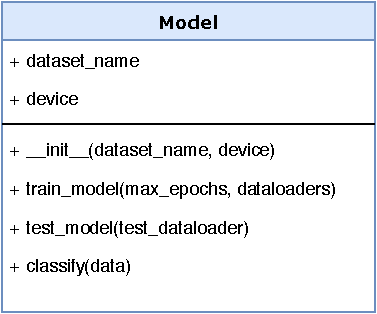
\includegraphics[scale=1]{figs/model_class.pdf}
  \caption{Model base class}
\end{figure}

The \texttt{dataset\_name} field is used to save the model state in the correct place when using early stopping, and the \texttt{device} field is 
used to ensure that GPUs are used if available. Not placing the tensors on the correct device 
leads to errors as PyTorch cannot perform operations on tensors located on different devices.

Each model has different fields depending on the structure of the model, so initialisation of the models could not be a general method. 
However, for evaluation I implemented a \texttt{hyperparameter\_loop} method per model 
which took the same arguments for all models:
\begin{center}
  \texttt{hyperparameter\_loop(fold, validation\_fold, state\_path, results\_path, dataset\_name, dataloaders, input\_size, num\_classes, max\_epochs, device)}
\end{center}

This method loops through a pre-selected set of hyperparameters to determine the best performing (Section ~\ref{hyper}).
This was possible because the hyperparameters chosen for searching over were not dependent on the input dataset, and were instead selected 
to give good general performance e.g. the ladder network hyperparameter search constructs ladder networks with 1-4 hidden layers, and
compares them, with the deeper model generally winning on more complicated datasets and the shallower on less complicated.

\subsection{Model training}

All the models were trained using mini-batch gradient descent, as described in Section~\ref{batch}.

\subsection{Multilayer perceptron}
The multilayer perceptron is a fully supervised model implemented to compare the performance between a fully supervised approach and the 
semi-supervised approaches used in the project. The model simply uses the Classifier base module and trains it on only the labelled data
using cross entropy loss~\eqref{eq:ce}.

\subsection{M1}
The M1 model described in Section~\ref{m1} It is made up of a VAE Encoder,
Decoder and Classifier 
module. The VAE Encoder and Decoder are initially trained in an unsupervised way using both the labelled and unlabelled data. In order 
to train them I made the decision to normalise all the data to the range [0-1] (Section~\ref{normalise}) and to use a Sigmoid function 
\footnote{the sigmoid function is of
the form $f(x) = \frac{1}{1+e^{-x}}$ and has the domain of the real numbers and range [0-1]} on the output of the Decoder, to ensure the output range 
was the same as the input. This was done for numerical stability reasons, as it was found that using unnormalised or standardised data 
as input to the VAE would cause the variance of the latent distribution to become infinitely small and eventually lead to the loss and 
output of the VAE becoming \texttt{nan}.

Once the VAE Encoder and Decoder are trained the Decoder is discarded. The labelled data is passed through the VAE Encoder, and the samples
from the distributions are used as input to the Classifier. The Classifier is then trained on this labelled data using cross entropy 
loss~\eqref{eq:ce}. 

This model relies on the manifold hypothesis. The training of the VAE hopefully clusters similar samples together by finding a lower
dimensional manifold, allowing the Classifier to more easily separate the classes using only a small amount of labelled data.

Once the Classifier is trained the full pipeline for classifying new data involves first passing the data 
through the VAE Encoder and then through the Classifier.

\begin{figure}[H]
  \centering
  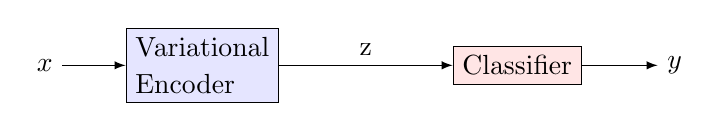
\begin{tikzpicture}
    \node at (0, 0) [black,] (x) {$x$};
    \node at (2, 0) [rectangle,draw,align=left,fill=blue!10] (vae_e) {Variational \\ Encoder};
    \node at (6, 0) [rectangle,draw,fill=red!10] (clas) {Classifier};
    \node at (8, 0) [black, ] (y) {$y$};
    \draw [->] (x) to (vae_e);
    \draw [->] (vae_e) to node[above] {z} (clas);
    \draw [->] (clas) to (y);
  \end{tikzpicture}
  \caption{The classification pipeline of the trained M1 model}
\end{figure}

\subsection{Stacked denoising autoencoder}
The SDAE was constructed by first constructing a list of one-layer Encoders. Each Encoder had the same input size as the latent dimension of the 
previous Encoder. All the Encoders use ReLU as the output activation function, and the final output layer is a simple \texttt{nn.Linear} layer with 
no output activation. This means that passing data through all the encoder followed by the output layer acts much like 
a Classifier module, but it enables easy unsupervised pretraining.

The unsupervised pretraining is performed by taking each encoder, starting with the first hidden layer, and adding the corresponding 
Decoder. This is where the pairing of the Encoder and Decoder is very useful, as by extracting the layer sizes of the Encoder they 
can be passed straight into the Decoder contructor to create the complementary Decoder. Then Gaussian noise is added to the input data,
using the PyTorch function \texttt{torch.randn\_like(data)}, which creates a Gaussian noise tensor of the same size as the data that can
simply be added to the data. This Encoder/Decoder pair is then trained like a normal autoencoder, training a single layer of the network.

Once each hidden layer has been trained like this, the whole network is trained using labelled data to optimise the network for the 
supervised learning task. Classification just involves passing the data through all the Encoders and then through 
the output layer.

\subsection{Semi-supervised VAE (M2)}

The M2 model (Section~\ref{ssVAE}) is made up of a Classifier, a Variational Encoder and a Decoder.
Data is first passed through the Classifier to get a prediction for the label. The loss functions used were given in Section~\ref{ssVAE}, 
and depend on whether the data is labelled or unlabelled. If the data is labelled then the data is passed into the Variational Encoder 
with the correct label, and the output of the Variational Encoder is passed into the Decoder which attempts to reconstruct the data.
If the data is unlabelled then the data and each possible label are passed into the Variational Encoder, and the reconstruction loss 
is computed for all the combinations. This seems like it would greatly increase the training time, but this can actually be done 
by creating a larger tensor with every unlabelled sample in the batch paired with each label. This operations on this larger tensor 
can be computed in parallel on the GPU so the performance hit is not as drastic as this operation might suggest. The code for performing this 
operation is:

{\renewcommand{\baselinestretch}{0.8}\small
    \begin{verbatim}
      def minus_U(self, x, pred_y):
        # gives probability for each label
        logits = F.softmax(pred_y, dim=1)

        # make a vector of length num_classes*batch_size with each 
        # label repeated batch_size times
        y = self.make_labels(x.size(0))
        # convert label vector to one-hot
        y_onehot = self.onehot(y)
        # repeat data num_classes times (x and y now have same length)
        x = x.repeat(self.num_classes, 1)

        # pass each datapoint with each label through encoder and decoder
        recons, mu, logvar = self.M2(x, y_onehot)
        
        # calculate labelled loss for each pair of datapoint and label (in parallel)
        minus_L = self.minus_L(x, recons, mu, logvar, y)
        # reshape output so all of num_class losses for each datapoint are together
        minus_L = minus_L.view_as(logits.t()).t()
        
        # multiply each labelled loss by the probability of the label
        minus_L = (logits * minus_L).sum(dim=1)

        # compute the entropy of the logits
        H = self.H(logits)

        # calculate -U
        minus_U = H + minus_L

      return minus_U.mean()
    \end{verbatim}
}

The overall structure of the model for unlabelled data is shown below. For labelled data the label passed into the Variational Encoder 
and Decoder comes from the dataset, not the classifier.

\begin{figure}[H]
  \centering
  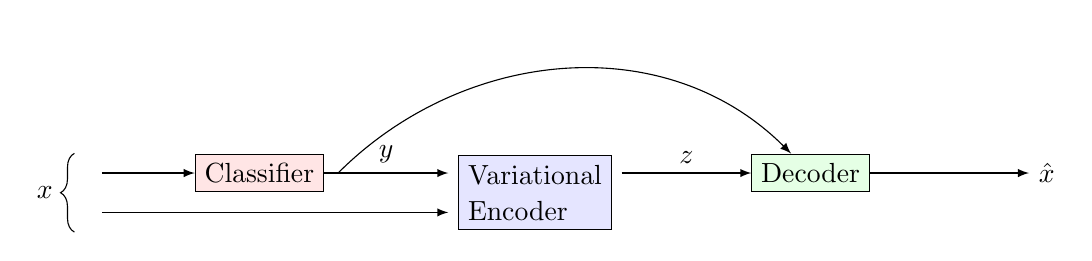
\begin{tikzpicture}
    \node at (2, 0.25) [rectangle,draw,fill=red!10] (clas) {Classifier};
    \node at (5.5, 0) [rectangle,draw,align=left,fill=blue!10] (vae_e) {Variational \\ Encoder};
    \node at (9, 0.25) [rectangle,draw,fill=green!10] (dec) {Decoder};
    \node at (12, 0.25) [black,] (x_hat) {$\hat{x}$};
    \draw [->] (0, 0.25) to (clas);
    \draw [->] (clas) to node[above] {$y$} (4.4, 0.25);
    \draw [->] (0, -0.25) to (4.4, -0.25);
    \draw [->] (6.6, 0.25) to node[above] {$z$} (dec);
    \draw [->] (3, 0.25) to[out=45,in=135] (dec);
    \draw [->] (dec) to (x_hat);
    \draw [decorate,decoration={brace,amplitude=5pt,mirror,raise=-1ex}]
      (-0.5,0.5) -- (-0.5,-0.5) node[left,midway]{$x$};
  \end{tikzpicture}
  \caption{Model structure of M2 for training on unlabelled data}
\end{figure}

The main diffculties in implementing this model came from conflicting information found online. 
The original paper~\cite{DBLP:journals/corr/KingmaRMW14} can be quite hard to decipher, often skipping over difficult derivations, and 
at one point seemingly contradicting itself on the structure of the model.
One of the original blog posts I viewed~\cite{Semisupe95:online} did not pass the label into the 
encoder, and after corresponding with the author I found it was due to a different interpretation of a line in the paper. However,
Kingma's implementation (available at: https://github.com/dpkingma/nips14-ssl) does pass the label into the encoder and so that is the 
model I followed. 

A helpful reference implementation I found is available at https://github.com/wohlert/semi-supervised-pytorch, but I believe my implementation is 
easier to read and also performs better, as I use the inbuilt PyTorch models for computing the cross entropy loss and use the Kingma way 
of computing the KLD~\cite{DBLP:journals/corr/KingmaW13}. I was able to contribute to the repository, finding a bug in the 
variational autoencoder code where the natural logarithm of the variance was restricted to values greater than zero (this is incorrect).

This model again requires that the data be normalised to the range [0-1] (as in M1) as otherwise the loss explodes and becomes 
\texttt{nan} as the variance of the latent distribution becomes very small.

Once the model is trained the only part used in classification is the Classifier.

\subsection{Ladder} \label{ladder_imp}

The ladder network doesn't make use of any of the base modules, as it requires a lot of extra parts. My original implementation 
was based on an implementation found at https://github.com/abhiskk/ladder. However, this implementation is very slow, as at one point 
tensors on the GPU are shifted onto the CPU to perform operations using numpy, which is unnecessary. The implementation also did 
not achieve the desired accuracy on MNIST. For this reason I instead based my implementation on a Tensorflow implementation written by 
Rinu Boney
(available at https://github.com/rinuboney/ladder), who works at Curious AI, the same company as Rasmus, the author of
the 2015 paper~\cite{DBLP:journals/corr/RasmusVHBR15}. The code required extensive rewriting to move from Tensorflow to PyTorch,
but my implementation is now the fastest and most accurate PyTorch implementation of the model I could find on the internet.

The model is described in some detail in Section~\ref{ladder}, and the overall training process is as below: 
\begin{enumerate}
    \item Data is passed into the clean encoder and the output from each layer is saved.
    \item Data is passed through the noisy encoder, and output from each layer is saved.
    \item The final output from the noisy encoder is the classification output, and supervised loss is computed with it.
    \item The output from the noisy encoder is fed into the decoder. At each layer $l$ of the decoder $g(\tilde{z}^{(l)}, u^{(l+1)})$ is calculated,
          and the unsupervised loss for the layer is computed.
    \item The unsupervised losses are multiplied by hyperparameter $\lambda_{l}$ and summed together.
    \item The supervised and unsupervised losses are summed and backpropagated through the network and the weights are updated.
\end{enumerate}

The Python code used to implement this process is:

{\renewcommand{\baselinestretch}{0.8}\small
    \begin{verbatim}
    for batch_idx, (labelled_data, unlabelled_data) in enumerate(
        zip(cycle(supervised_dataloader), unsupervised_dataloader)):
    self.ladder.train()

    self.optimizer.zero_grad()

    labelled_images, labels = labelled_data
    labelled_images = labelled_images.to(self.device)
    labels = labels.to(self.device)

    unlabelled_images, _ = unlabelled_data
    unlabelled_images = unlabelled_images.to(self.device)

    inputs = torch.cat((labelled_images, unlabelled_images), 0)

    batch_size = labelled_images.size(0)
    
    # pass data through encoders clean
    y, clean = self.ladder.forward_encoders(inputs, 0.0, True, batch_size)
    # pass data through encoders noisy
    y_c, corr = self.ladder.forward_encoders(inputs, self.noise_std, True, batch_size)

    # compute supervised cross entropy loss
    supervised_cost = self.supervised_cost_function.forward(labeled(y_c, batch_size), 
                                                            labels)
    
    # pass output of encoder through decoder
    z_est_bn = self.ladder.forward_decoders(F.softmax(y_c), corr, clean, batch_size)
    zs = clean['unlabeled']['z']
    
    # compute unsupervised reconstruction loss for each layer
    unsupervised_cost = 0
    for l in range(self.L, -1, -1):
        unsupervised_cost += self.unsupervised_cost_function.forward(
            z_est_bn[l], zs[l]) * self.denoising_cost[l]
     
    loss = supervised_cost + unsupervised_cost
    
    # backpropagate loss through network and update weights
    loss.backward()
    self.optimizer.step()
    \end{verbatim}
}

For the most part this was implemented without difficulty, though I did discover early on that the loss sometimes became \texttt{nan}.
By adding a backward hook to the model that would notify me when the values became \texttt{nan} I discovered that this was due to the 
fact that the ladder requires the data be standardised (Section~\ref{normalise}), which involves dividing the features in the data by the standard deviation of the 
features. However, in the MNIST dataset the pixels on the edge of the images are always black, and so have a constant value of zero over 
all the images. The standard deviation of these features is therefore also zero, and dividing by this leads to data becoming \texttt{nan}.
This can be fixed by adding a small positive value to the denominator when standardising.

\section{Hyperparameter optimisation} \label{hyper}
While the weights and biases in a network can be trained by backpropagation, there are parameters of the model that cannot be trained in 
this way, but still affect the performance of the network. These are hyperparameters and they are set before the training begins. 
Optimising these can be crucial in getting the best performance from a model.

\subsection{Grid search}
The most common method for hyperparameter optimisation, and the one used in this project, is grid search. The researcher provides several 
likely values for the hyperparameters, and the model is trained with each combination of these. A validation set is used to compare the
performance of the models, and the best set of hyperparameters is selected this way.

However, optimising hyperparameters this way results in every combination having to be run again for each additional value of each
hyperparameter used. Depending on how long it takes each model to train, this can result in hours more training time. 
Therefore, I chose to optimise over a small number of hyperparameters that I felt were most likely to affect the performance of the models.

\subsection{Number of hidden layers}
The number of layers in a model is important because it controls the capacity~\cite{Goodfellow-et-al-2016} of the neural network. If the 
capacity of the network is too high it can \textbf{overfit} to the training data, resulting in poor generalization to new examples, and if the capacity is 
too low it can \textbf{underfit}, resulting in poor fitting to the train data. Therefore choosing the number of layers is an important hyperparameter.
The universal approximation theorem states that a neural network with a single hidden layer can approximate any function~\cite{DBLP:journals/mcss/Cybenko92}, but the layer 
has to be exponentially large to give the same capacity as a multi-layer network; instead adding new layers is the preferred method, 
with the deeper layers learning more complex and relevant features to the task.

\subsection{Hidden layer size}
Larochelle et al.~\cite{DBLP:journals/jmlr/LarochelleBLL09} found that neural networks with constant layer size usually perform better than
those where the layer size increases or decreases throughout the network. When optimising the number of layers I use a constant layer size
for each hidden layer.

Bengio et al.~\cite{DBLP:series/lncs/Bengio12} found that using a first hidden layer larger than the input layer often resulted in 
better performance. However due to the high dimensionality of gene expression data (over 20,000 genes in the TCGA data) I decided against 
this. I use a constant layer size for all the hidden layers, using the same layer size for all the different models to allow for a fairer
comparison.

\subsection{Latent dimension of autoencoders}
The size of the latent dimension for an autoencoder affects the quality of the representation learned. If the dimension is too small the 
autoencoder may not be able to encode all the important features, whereas a latent dimension that is too large can give the autoencoder 
too much freedom, causing it to not cluster important samples together.

This hyperparameter is only optimisable for the M1 and M2 models, as the hidden dimensions for the autoencoder in the SDAE and ladder 
are controlled by the layer size and number of classes.

\subsection{Learning rate}
The learning rate is a hyperparameter that controls how large of a step is taken each time the weights are updated. It is an often
optimised hyperparameter because if it is too large it can overshoot loss minima, resulting in worse performance, and if it is too 
small it can take a very long time for the gradient descent to converge. However, I have chosen not to search over different learning 
rates because of the additional time it would take, and the fact that I am using the \textbf{Adam optimizer}. The Adam optimizer keeps a 
learning rate per parameter, and updates these learning rates according to the first and second moments of the gradients with respect to each 
parameter~\cite{DBLP:journals/corr/KingmaB14}. This means that while an initial learning rate still has to be provided, it affects the 
performance much less.

\subsection{Early stopping}
The number of epochs that a learning algorithm is trained for also affect how well it performs. Not training for long enough can result in
poor peformance and underfitting, as the model has not had enough time to learn the relevant features, while training for too long can
be wasted compute time if the model is not improving, or even lead to overfitting.

Luckily, this is one of the easiest hyperparameters to optimise, and does not have to be included in a grid search. 
With the use of a validation set that the network is not trained on the performance of each model on unseen data can be measured after 
every epoch. Unseen data is necessary because evaluating a model on training data will give overfitted models excellent performance, 
while the actual model generalises poorly and is unusable.
If the performance has improved the state of the model is saved. After a certain number of epochs without the performance improving 
the training is stopped, and the best performing model state is loaded.

\section{Data processing}
An important part of a machine learning project is the pre-processing of the data. This is used to ensure good model performance and 
to partition the data to allow unbiased evaluation.

\subsection{Datasets}
\subsubsection{MNIST handwritten digit database}
The MNIST dataset is one of the most popular in machine learning, being used to benchmark new models is many papers.
\begin{table}[H]
  \label{tab:mnist}
  \small % text size of table content
  \centering % center the table
  \begin{tabular}{lccr} % alignment of each column data
  \toprule[\heavyrulewidth]
  Samples & 60,000 train \& 10,000 test \\
  Inputs & 28x28 b/w images  \\
  Number of classes & 10 - digits 0-9 \\
  Balanced & Yes \\
  \bottomrule[\heavyrulewidth] 
  \end{tabular}
  \caption{MNIST dataset} 
\end{table}

In this project it is again used for benchmarking, and for ensuring that the models are performing similarly to their original implementations.

\subsubsection{The Cancer Genome Atlas}
The Cancer Genome Atlas is a project cataloguing sequencing data for several different types of cancer. The data generated by the TCGA Research 
Network (https://www.cancer.gov/tcga) is available online at https://portal.gdc.cancer.gov. In this project I used data generated using 
RNA-Seq to attempt to classify the different types of cancer using only their gene expression.
\begin{table}[H]
  \label{tab:tcga}
  \small % text size of table content
  \centering % center the table
  \begin{tabular}{cc} % alignment of each column data
  \toprule[\heavyrulewidth]
  Samples & 11,060 \\
  Inputs & 20,350 genes with values given as $\log_{2}(\text{TPM}+1)$ \footnotemark \\
  Number of classes & 33 - different cancer types\\
  Balanced & No \\
  \bottomrule[\heavyrulewidth] 
  \end{tabular}
  \caption{MNIST dataset} 
\end{table}
\footnotetext{TPM is transcripts per million, where the total number of reads mapped to a gene is normalised by the length of the gene} 

\subsection{Data normalisation} \label{normalise}
Data normalisation can help neural networks by allowing gradient descent to reach a minima more easily. Features having large ranges
can result in larger gradients of the loss, resulting in larger steps being taken at the weights. This can cause the 
gradient descent to oscillate around minima and take far longer to reach a good value. The two most common forms of data normalisation 
are standardisation and normalisation to the range [0-1]. Having all the features with similar scales is also important for saliency computation
(Section~\ref{saliency}),
as different scales result in different gradients of the output with respect to the input, preventing them from being directly comparable.

\begin{itemize}
  \item \textbf{Standardisation} involves scaling all the features so that they have mean 0 and variance 1. This is done be computing the mean 
          and standard deviation of the features from the training set, and then subtracting the mean from each feature and dividing by the
          standard deviation.
          \begin{align}
            x_{std} = \frac{x - \mu_{x}}{\sigma_{x}}
          \end{align}
  \item \textbf{Normalisation} into the range [0-1] is done by finding the maximum and the minimum for every feature from the training set,
          subtracting the minimum from every feature and dividing by the maximum minus the minimum.
          \begin{align}
            x_{norm} = \frac{x - x_{max}}{x_{max} - x_{min}}
          \end{align}
\end{itemize}

For the MNIST dataset I used normalisation, as the pixels take values between 0 and 255 and so scaling this to be between 0 and 1 is 
a simple and intuitive transform. It is also the transform used in the code for the ladder network paper~\cite{DBLP:journals/corr/RasmusVHBR15}, 
and similar to the transform used in the semi-supervised VAE paper~\cite{DBLP:journals/corr/KingmaRMW14} (here they set pixel values to 
either zero or one, without the range inbetween).

For the gene expression datasets I tried both standardisation and normalisation. Standardisation worked well for the non-VAE based models,
but the M1 and M2 models experienced significant numeric instability. This is a somewhat common problem in
VAEs, especially when the dimensionality of the data is higher than the number of samples in the dataset. The VAEs responded well to normalised
data, while the other models experienced similar or worse performance. Therefore standardisation was used for the MLP, SDAE and ladder 
network and normalisation was used for M1 and M2.

\subsection{Data imputation} \label{imput}
The TCGA dataset contains the gene expression levels for 20,350 genes, but in many of the samples some of these genes are missing.
This can be dealt with by simply discarding the samples with missing genes, but this can be a significant number of samples, and removing 
a large chunk of the dataset is not a good way to improve a model. Instead it may be possible to impute the missing genes, or drop the 
genes entirely, reducing the number of features but keeping the number of samples. In Section~\ref{imputation} there is a comparison 
of the performance of dropping the genes, replacing the missing values with the feature mean, and replacing the missing values with zero.

\subsection{Data partitioning} \label{part}
\subsubsection{Evaluating models and hyperparameter optimisation}
Evaluating the performance of a machine learning algorithm should be done on a test dataset that is separate from the dataset the 
algorithm is trained on, to prevent overfitting leading to overestimating the performance of the model. If the dataset is not particularly 
large this can be done using 
\textbf{$k$-fold cross validation}, where the data is split into $k$ different partitions. $k-1$ of these partitions are used for training, 
while the $kth$ is used to test the performance after training. The accuracy for the model is then computed by taking the average of all
the accuracies for each fold.

\begin{figure}[H]
  \centering
  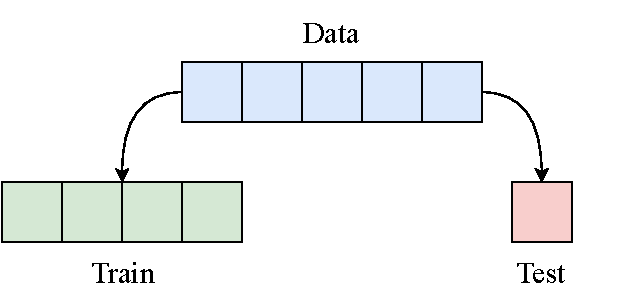
\includegraphics[scale=0.75]{figs/k_fold.pdf}
  \caption{One split of 5-fold cross validation}
\end{figure}

The $k$-fold cross-validation used in this project is \textbf{stratified}. This keeps the proportion of each class in each fold
close to the proportion of each class in the overall dataset. This is especially important when classes are unbalanced, as performing 
non-stratified cross-validation could result in biasing the model towards an uncommon class, or not including any samples of a class in the 
fold. It has been shown by Kohavi~\cite{Kohavi:1995:SCB:1643031.1643047} stratified cross-validation generally has lower bias and variance when estimating model 
accuracies.

In order to perform hyperparameter optimisation (Section~\ref{hyper}) there needs to be a validation dataset, to 
compare the performance of each set of hyperparameters. Performing hyperparameter optimisation on the test set will lead to overestimating 
the ability of the model to perform on unseen data, as the hyperparameters have been chosen to perform best on the test set. Therefore,
another split has to be made to generate a validation set. The most common way to do this is \textbf{nested k-fold cross validation}:
partition the training data into another $k$ folds; compute the validation performance for each set of hyperparameters $k$ times; take the 
hyperparameters that perform best on average and train a model with those hyperparameters on all the training data.
However this method has a couple of problems. Firstly if there are $n$ hyperparameter sets to test over this method will take $nk^{2}$ 
iterations, and even if a model is quick to train the time this takes quickly becomes very large. It also means that there is no validation set used 
for the final computation of the model. As I am using early stopping a validation set is always required because the number of epochs 
to train to get best performance can be quite variable and depend on the model weight initialisation.

Therefore I instead partitioned the $kth$ fold in two, into a validation set and a test set. The hyperparameters are optimised using the 
validation set, and the performance of each model is compared. The best performing model is then run on the test set and the acccuracy
recorded. The test and validation sets are then swapped and optimisation is performed again. This reduces the number of iterations to
$2nk$ and also ensures that there is always a validation set to perform early stopping, while still using all the available data as train, 
validation, or test data at some point.
\begin{figure}[H]
  \centering
  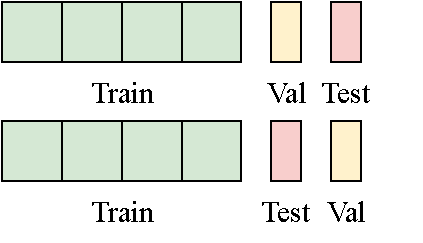
\includegraphics[scale=0.75]{figs/test_val_split.pdf}
  \caption{Splitting test set into a test and val set for hyperparameter optimisation}
\end{figure}

\subsubsection{Labelled splits}
While the datasets used in this project include labels for all the samples, the focus of this project is on semi-supervised learning.
In order to give an overall view of the performance for each dataset I performed evaluation of the models with different amounts of
labelled data. For each number of labelled samples ($n$) used, I selected $n$ samples from the train set in a stratified way to use as the 
labelled dataset. The unlabelled dataset was then all the remaining samples in the train set.

\subsubsection{Parallelisation}
While the cross-validation changes made above reduce the number of iterations to a more manageable size, even a model with a fairly short 
training time will take a long time to complete the evaluation. To this end I computed the indices of test/val/train and labelled 
splits I would use in advance, and serialised these using \texttt{pickle} \footnote{\texttt{pickle} is the most popular Python library 
for serialisation}. This allows all the models to use the exact same folds, allowing
for a fair comparison. It also allows each script to run hyperparameter optimisation over only one fold. The Cambridge High Performance
Cluster has 90 GPUs, and so running many smaller jobs in parallel results in a much quicker finish time than running several larger jobs.
To this end I also wrote several \texttt{bash} scripts to schedule slurm jobs for each model, number of labelled examples and fold. 

\section{Saliency} \label{saliency}
Neural networks often act as a black box, with no indication to the programmer or user of what the network is doing, and what it deems 
to be important. One way of extracting that is through the use of saliency maps (first introduced in~\cite{DBLP:journals/corr/SimonyanVZ13}), 
which intend to give the user some idea of which inputs 
are the most important in determining the output class. The way this is done is by computing the partial derivatives of the input data 
with respect to the output class of the network. If the input values have been scaled to have similar ranges then this partial derivative
should be larger for for inputs that are more important to determining the class. A large positive partial derivative means that increasing 
the value of that input makes the class more likely, and a large negative partial derivative means increasing that input decreases the 
likelihood of that class.

A variant of this uses guided backpropagation~\cite{DBLP:journals/corr/SpringenbergDBR14}, a variant of backpropagation where the 
gradient is only backpropagated through a ReLU if the error gradient is greater than zero. When used to construct saliency maps for 
images it has been shown to make much clearer images, and highlight better the features the network thinks are important.

I implemented both of these methods, basing my implementation on this very simple implementation: https://github.com/Ema93sh/pytorch-saliency.
The guided backpropagation version works by registering a hook on each ReLU module that sets the gradient being backpropagated through it 
to zero if it is less than zero.

\section{Command line tool}
One of the success criteria of this project was to build a tool, and so the \texttt{main.py} file in the repository provides a command line tool 
for building a semi-supervised learning model. The tool uses many of the techniques described earlier in this section, but many of the 
decisions made are based on results in the evaluation section, so the description of the tool is available in Section~\ref{tool}.

\section{Repository overview}

\begin{figure}[H]
    \centering
    \begin{minipage}{7cm}
        \dirtree{%
        .1 +Semi-Supervised\_Models.
        .2 main.py.
        .2 requirements.txt.
        .2 +Models.
        .3 Model.py.
        .3 Simple.py.
        .3 M1.py.
        .3 SDAE.py.
        .3 M2.py.
        .3 Ladder.py.
        .3 +BuildingBlocks.
        .2 Saliency.
        .2 scripts.
        .2 utils.
        }
    \end{minipage}
    \caption{Directory structure of the repository}
\end{figure}

The top level of the repository contains the files \texttt{main.py} and \texttt{requirements.txt}. These are the script for running the tool,
and the packages I am using in the virtual environment respectively. \texttt{Models} contains all the code for the models used in this project,
including the base modules in \texttt{BuildingBlocks} and the abstract class \texttt{Model.py}.
\texttt{scripts} contains all the python and bash scripts used in 
obtaining the results for the evaluation section, but this folder was created for tidiness and the scripts have to be moved up one level into 
\texttt{Semi-Supervised\_Models} to be run. \texttt{utils} contains functions for loading data, along with the code for early stopping and 
making the MNIST and TCGA folds. \texttt{Saliency} contains all the code for generating saliency maps.

\chapter{Evaluation}

\textit{In this section I will compare the performance of the semi-supervised models on both the MNIST and TCGA datasets, and will compare these 
to a fully supervised MLP operating on only the labelled data. I then discuss how these factored into the choices made for a more general
tool. All the results in this section can be replicated using the Python and bash scripts found in the scripts folder}

\section{MNIST}

\subsection{Semi-supervised results}
The MNIST results are important for establishing whether the ladder and M2 models have been correctly implemented, as they should 
achieve close to paper accuracy. It should also give some indication of how the models are expected to perform on the gene expression data.

The MNIST dataset has a designated train and test set, so to obtain the results for this I performed 5-fold cross validation over the 
training set, using 48,000 examples for testing and 12,000 for validation and then computing the accuracy of the model on the 10,000
test samples. Accuracy is computed as the number of datapoints in the test set where the label was correctly predicted divided by the 
total number of datapoints in the test set, given below as a percentage of points correctly classified.
\begin{table}[H]
  \label{tab:mnist}
  \small % text size of table content
  \centering % center the table
  \begin{tabular}{R|CCCCC} % alignment of each column data
  \toprule[\heavyrulewidth]\toprule[\heavyrulewidth]
  & \multicolumn{5}{c}{\textbf{Models}}\\
  \shortstack{Number of \\ labelled samples} & \textbf{MLP} & \textbf{SDAE} & \textbf{M1} & \textbf{M2} & \textbf{Ladder} \\ 
  \midrule
  100 & 71.75 \pm 0.82 & 74.86 \pm 0.85 & 49.00 \pm 0.98 & 92.34 \pm 0.52 & 96.64 \pm 0.35\\
  1000 & 88.86 \pm 0.62 & 91.97 \pm 0.53 & 83.44 \pm 0.73 & 96.57 \pm 0.36 & 98.03 \pm 0.27\\
  3000 & 93.88 \pm 0.47 & 95.60 \pm 0.40 & 88.55 \pm 0.62 & 97.19 \pm 0.32 & 98.35 \pm 0.25\\
  \text{All} & 98.41 \pm 0.25 & 98.58 \pm 0.23 & 90.30 \pm 0.58 & 98.45 \pm 0.24 & 98.95 \pm 0.20\\
  \bottomrule[\heavyrulewidth] 
  \end{tabular}
  \caption{MNIST 5-fold cross-validation percentage accuracies} 
\end{table}

\subsubsection{Performance comparisons}
The MLP and SDAE do not have standard accuracies that can be obtained from papers, but the slight performance boost the SDAE provides 
over the MLP when only some of the data is labelled is what was expected.

The results for M1 are much worse than those in the original Kingma paper~\cite{DBLP:journals/corr/KingmaRMW14}, and this is due to the use
of a neural network as the classifier on the latent dimension. This neural network can only use the labelled samples, while the Kingma 
paper uses a transductive support vector machine, which is able to utilise the unlabelled samples in seperating the classes. In order to
not overcomplicate the project I decided against implementing a TSVM and so the results are poor. Part of the reason the results are worse 
than even the basic MLP are that the supervised learning cannot effect the weights of the VAE. If the VAE is encoding useless information 
the supervised update steps are unable to prevent this.

The results for M2 are comparable to those in the Kingma paper, and for the 100 labelled samples are actually better, averaging 92.34 
compared to 88.03. I believe that these improvements are due to performing hyperparameter optimisation over the latent dimension of the 
model, whereas the Kingma paper used a fixed latent size of 50.

The ladder results are again comparable, with my implementation averaging 96.64 compared to 98.94 by Rasmus~\cite{DBLP:journals/corr/RasmusVHBR15}
for 100 labelled samples.
The discrepancy is likely due to the slight differences in model structure. I optimise over 1 to 4 hidden layers of fixed size,
while Rasmus uses 5 hidden layers with an overcomplete (1000 neurons) first hidden layer.

\subsection{Saliency}

Saliency maps computed using both normal and guided backpropagation are below, demonstrating how the models learn the important 
sections of the image for classifying.

\begin{figure}[H]
  \centering
  \begin{subfigure}[b]{0.4\linewidth}
    \centering
    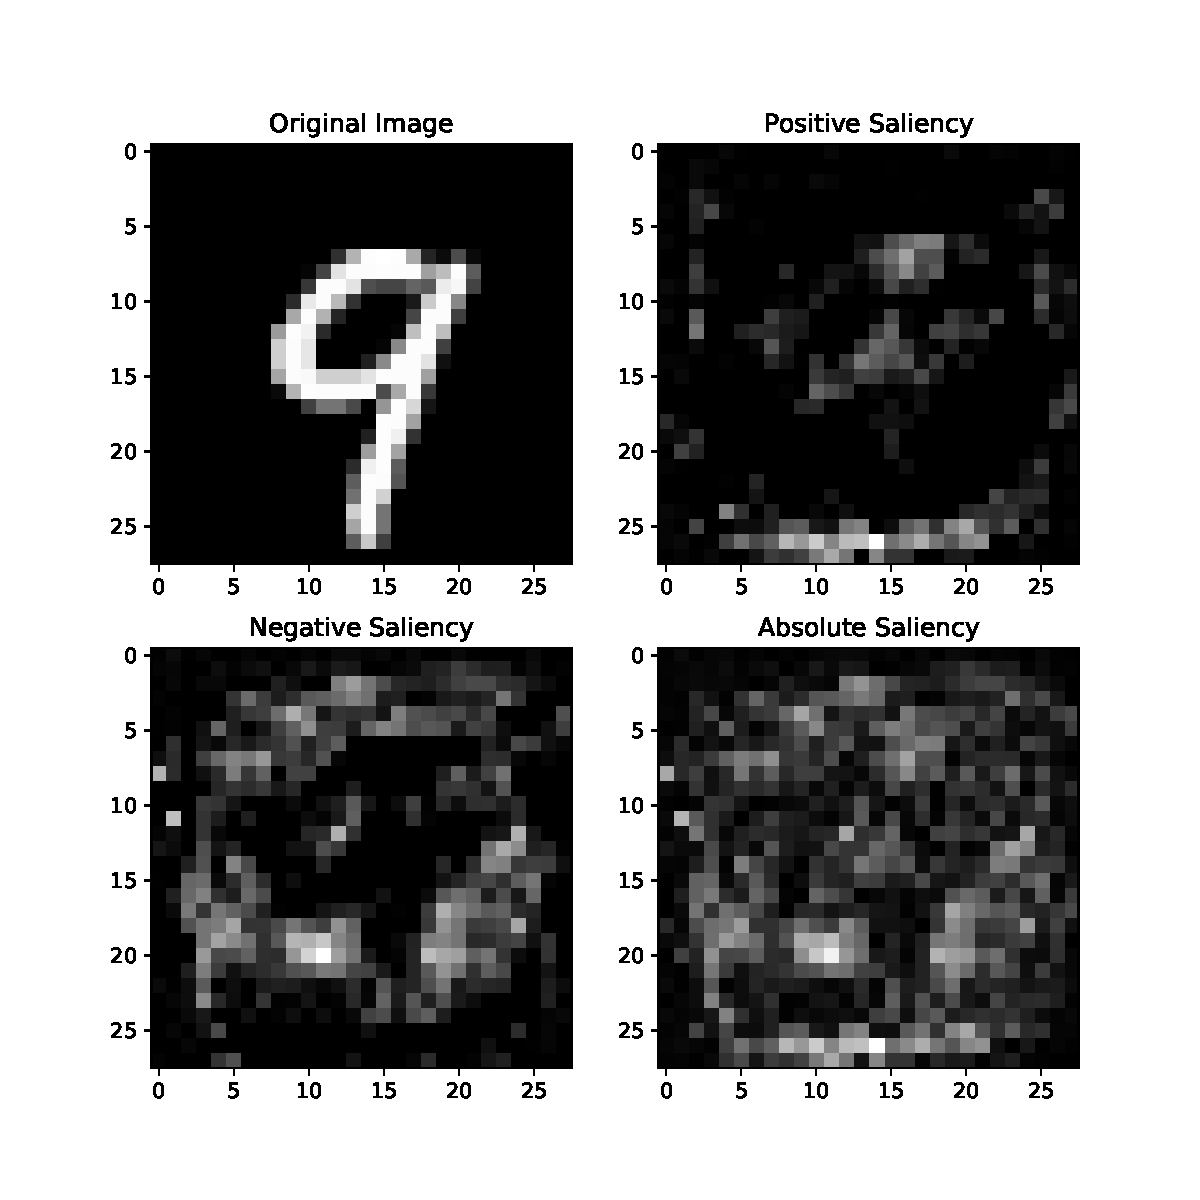
\includegraphics[scale=.25]{figs/vanilla_saliency_maps.pdf}
    \caption{Vanilla saliency}
  \end{subfigure}
  \begin{subfigure}[b]{0.4\linewidth}
    \centering
    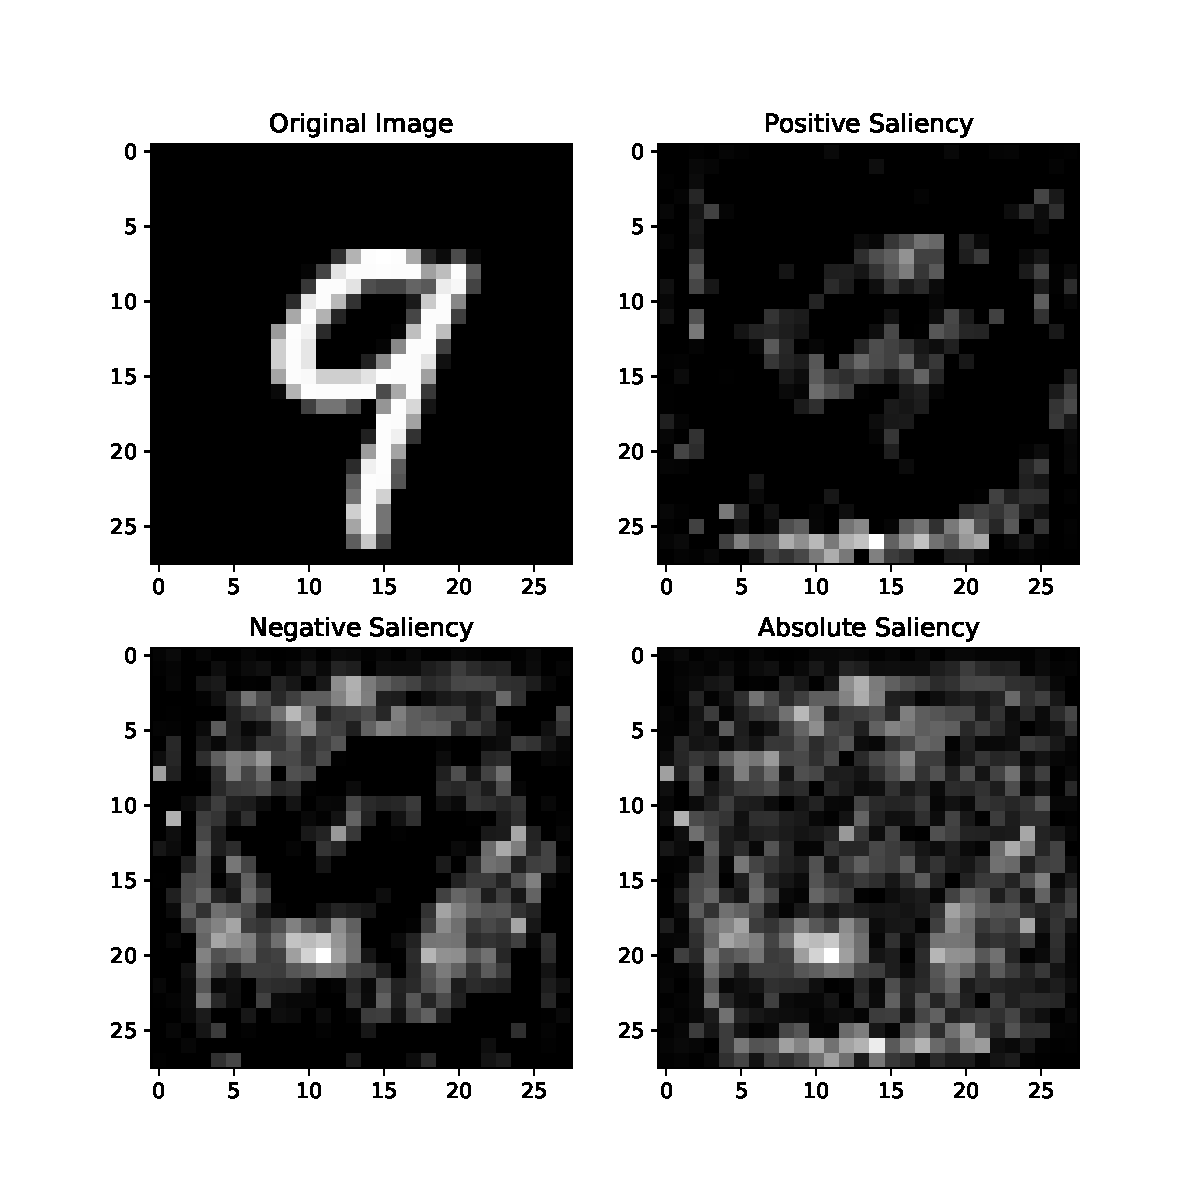
\includegraphics[scale=.25]{figs/guided_saliency_maps.pdf}
    \caption{Guided saliency}
  \end{subfigure}
  \caption{Saliency maps for 9}
  \label{fig:saliency}
\end{figure}

The difference between the two saliency types is subtle, but the guided saliency maps are generally less noisy than the vanilla saliency.
There is a clear outline of the top of a 9 in the positive saliency maps, and the high scoring pixels in the negative saliency maps would transform 
it into an 8 or possibly a 4. In this way these maps allow a user to understand what inputs are important for the network classification.

\section{TCGA results}

\subsection{Missing data} \label{imputation}

As some of the samples in the TCGA dataset are missing expression levels for certain genes I decided to compare the results (using an MLP 
and all of the data as labelled data) of three different techniques for removing the missing values. The first technique was to just drop
all the columns of genes with any missing values, reducing the number of genes from 20,350 to 16334. The second technique involved 
replacing all the missing gene expression values with zero, and the third involved replacing them with the mean of the expression 
level for all the samples. The results are summarized in the table below:
\begin{table}[H]
  \label{tab:imputation}
  \small % text size of table content
  \centering % center the table
  \begin{tabular}{CCC} % alignment of each column data
  \toprule[\heavyrulewidth]\toprule[\heavyrulewidth]
  \textbf{Drop genes} & \textbf{Zero} & \textbf{Mean} \\ 
  \midrule
  95.09 \pm 0.40 & 95.67 \pm 0.38 & 95.81 \pm 0.37 \\
  \bottomrule[\heavyrulewidth] 
  \end{tabular}
  \caption{TCGA data imputation 10-fold cross-validation percentage accuracies} 
\end{table}

Computing a paired t-test helps discern if any one method could be considered better.
\begin{table}[H]
  \label{tab:ttest}
  \small % text size of table content
  \centering % center the table
  \begin{tabular}{CCC} % alignment of each column data
  \toprule[\heavyrulewidth]\toprule[\heavyrulewidth]
  \textbf{Mean/Drop genes} & \textbf{Mean/Zero} & \textbf{Drop genes/Zero} \\ 
  \midrule
  1.723 & 0.543 & -1.753 \\
  \bottomrule[\heavyrulewidth] 
  \end{tabular}
  \caption{t statistics for difference between imputation folds} 
\end{table}

None of these t statistics are statistically significant using a two-tailed t-test with p=0.05, and so we cannot reject the null hypothesis
that all the imputation methods have the same performance. However, dropping the genes makes the least sense, as that way some real data is
lost.

\subsection{Semi-supervised results}

The results in this section were obtained by computing cross-validation as in Section~\ref{part}. All samples with missing data were 
dropped from the dataset to avoid bias due to the imputation type. 

One caveat with these results is that they represent an upper bound on the performance of the models, as a validation set is used that is 
sometimes larger than the number of labelled examples in the training set. This is obviously not feasible in real life, and so the 
results when used in a production setting will likely not be as good. However, this validation set was required for a fair comparison,
as the number of layers and epochs that get the best performance from each model greatly differs from model to model.

\subsubsection{Accuracy}

\begin{table}[H]
  \label{tab:tcga_acc}
  \small % text size of table content
  \centering % center the table
  \begin{tabular}{R|CCCCC} % alignment of each column data
  \toprule[\heavyrulewidth]\toprule[\heavyrulewidth]
  & \multicolumn{5}{c}{\textbf{Models}}\\
  \shortstack{Number of \\ labelled samples} & \textbf{MLP} & \textbf{SDAE} & \textbf{M1} & \textbf{M2} & \textbf{Ladder} \\ 
  \midrule
  100 & 77.54 \pm 0.85 & 78.69 \pm 0.84 & 68.83 \pm 0.95 & \textbf{90.92} \pm 0.59 & 87.56 \pm 0.67\\
  500 & 91.09 \pm 0.58 & 91.32 \pm 0.57 & 91.08 \pm 0.58 & \textbf{93.73} \pm 0.49 & 93.26 \pm 0.51\\
  1000 & 93.02 \pm 0.52 & 93.53 \pm 0.50 & 92.20 \pm 0.55 & 93.90 \pm 0.49 & \textbf{94.08} \pm 0.48\\
  \text{All} & 96.47 \pm 0.37 & 96.13 \pm 0.39 & 93.67 \pm 0.50 & 96.53 \pm 0.37 & \textbf{96.69} \pm 0.37\\
  \bottomrule[\heavyrulewidth] 
  \end{tabular}
  \caption{TCGA 10-fold cross-validation percentage accuracies} 
\end{table}

As can be seen from the results in the table there is no performance benefit in using the M1 model over the simple MLP, but the accuracy 
achieved nevertheless shows that M1 is probably learning an informative manifold. The SDAE shows a slight performance advantage, but 
clearly performs less well than M2 and the ladder.

The ladder and M2 both show a significant performance advantage over the MLP, and by computing the a t-test between the three models 
it can be shown which models perform statistically better with each amount of labelled data. 
\begin{table}[H]
  \label{tab:tcga_ttest}
  \small % text size of table content
  \centering % center the table
  \begin{tabular}{R|CCC} % alignment of each column data
  \toprule[\heavyrulewidth]\toprule[\heavyrulewidth]
  \shortstack{Number of \\ labelled samples} & \textbf{MLP/M2} & \textbf{MLP/Ladder} & \textbf{M2/Ladder} \\ 
  \midrule
  100 & -20.61 & -13.40 & 5.36 \\
  500 & -7.86 & -6.47 & 1.98 \\
  1000 & -2.89 & -4.59 & -1.41 \\
  \text{All} & -0.30 & -2.36 & -1.03 \\
  \bottomrule[\heavyrulewidth] 
  \end{tabular}
  \caption{TCGA 10-fold t-statistics between MLP, ladder and M2} 
\end{table}

The significance threshold for a two fold t-test, using  p=0.05 and 9 degrees of freedom, is 2.26. Therefore, looking at these results 
the ladder network significantly outperforms the MLP at every amount of labelled data. The M2 model outperfoms the MLP significantly 
until all the data is labelled. At this point the performance should be almost exactly the same as the MLP, as the training of the 
classifier in the M2 model is only controlled by the supervised cross entropy loss. The ladder is outperformed by the M2 model with 100
labelled samples, but with more labelled samples the difference between them is not statistically significant.

\subsubsection{Matthews correlation coefficient}

Accuracy is not always the best metric to use when evaluating a machine learning model, expecially when the classes in the model are 
imbalanced, as it can mean that predicting just the most populous classes results in good accuracy. For binary classification one of the 
preferred methods is using the Matthews correlation coefficient, which is regarded as 
a balanced measure even when the classes are unbalanced because it takes into account the balance ratios of the four possible 
categories (true positive, true negative, false positive, false negative)~\cite{Chicco2017}. There is a multiclass variant of this 
coefficient that ranges between a minimum value of between $-1$ and $0$
(depending on the distribution) and $+1$, with $+1$ meaning perfect correlation between the predicted and actual labels and $0$ meaning no 
correlation. This is calculated as below for $k$ classes: 

\begin{align}
  \text{MCC} = \frac{\sum_{k}\sum_{l}\sum_{m} C_{kk}C_{lm} - C_{kl}C_{mk}}{
  \sqrt{
  \sum_{k}(\sum_l C_{kl} )(\sum_{k' | k' \neq k}\sum_{l'} C_{k'l'})
  }
  \sqrt{
  \sum_{k}(\sum_l C_{lk} )(\sum_{k' | k' \neq k}\sum_{l'} C_{l'k'})
  }
  }
\end{align}

Calculating this for M2 and the ladder network gives:
\begin{table}[H]
  \label{tab:mcc}
  \small % text size of table content
  \centering % center the table
  \begin{tabular}{R|CC} % alignment of each column data
  \toprule[\heavyrulewidth]\toprule[\heavyrulewidth]
  \shortstack{Number of \\ labelled samples} & \textbf{M2} & \textbf{Ladder} \\ 
  \midrule
  100 & 0.9041 & 0.8683 \\
  500 & 0.9337 & 0.9286 \\
  1000 & 0.9354 & 0.9372 \\
  \text{All} & 0.9631 & 0.9649\\
  \bottomrule[\heavyrulewidth] 
  \end{tabular}
  \caption{Multiclass Matthews correlation coefficient} 
\end{table}

This is actually not much more informative than the accuracy scores, giving very similar results.

\subsubsection{Confusion matrix}

Viewing the confusion matrix can sometimes give a better insight into where a model is successful and unsuccessful. A confusion
matrix has the actual labels on the y-axis and the predicted labels on the x-axis. Each cell contains the number of datapoints with the 
real label on the y-axis that have been predicted the label on the x-axis.

The confusion matrices for the TCGA data are very large due to the large number of classes in the data, and so are included in Appendix~\ref{confusion} 
where they can be viewed in larger size.

Both the ladder and M2 matrices are very similar, and show the same weaknesses. \textit{Rectum adenocarcinoma} 
is misclassified almost 
100\% of the time by both models, as it is a very similar cancer to \textit{colon adenocarcinoma}, with both being the same type of cancer
occuring in a very similar location in the body. The other often misclassified cancers include \textit{brain lower grade glioma} and 
\textit{glioblastoma mutliforme}, both gliomas located in the brain with differing severity, and \textit{uterine carcinosarcoma} and 
\textit{uterine corpus endometriod carcinoma}. 

The difficulty in classifying these using gene expression is to do with the similarities in gene expression within cells of a certain tissue.
There is also the fact that the boundary between the grades of cancer cannot always be well defined, depending on a range of factors 
including rate of growth and necrosis that can cause the cancer to move between grades.

However, when the number of labelled examples is increased these misclassifications are reduced, with only the rectum and colon adrenocarcinoma 
significantly misclassifed with all the labels.

\subsubsection{Ensemble learning} \label{ensemble}

One way of improving the performance of a classification model is combining the classifications of two different models which may have learned
slightly different features and class boundaries. The combination of the models can then lead to an improvement in the accuracy as the 
different features and boundaries can combine to make a better classifier. The simplest way of doing this is to take the softmax 
output of the different models and sum them together. Dividing by the number of models then gives a new probability distribution that is the
average of the previous models. Taking the maximum of this distribution is the predicted label, and if the models have learned complementary
features this will improve the accuracy. Combining the M2 and ladder predictions produces the results below:
\begin{table}[H]
  \label{tab:ensemble}
  \small % text size of table content
  \centering % center the table
  \begin{tabular}{R|CC} % alignment of each column data
  \toprule[\heavyrulewidth]\toprule[\heavyrulewidth]
  \shortstack{Number of \\ labelled samples} & \textbf{Accuracy} & \textbf{MCC} \\ 
  \midrule
  100 & 90.89 \pm 0.59 & 0.9036 \\
  500 & 94.00 \pm 0.49 & 0.9365 \\
  1000 & 94.22 \pm 0.48 & 0.9388 \\
  \text{All} & 96.82 \pm 0.36 & 0.9662 \\
  \bottomrule[\heavyrulewidth] 
  \end{tabular}
  \caption{Accuracy and MCC for an average of M2 and ladder} 
\end{table}

These results are statistically significant improvements over M2 and the ladder network for different amounts of labelled data.

\begin{table}[H]
  \label{tab:tcga_ensemble}
  \small % text size of table content
  \centering % center the table
  \begin{tabular}{R|CC} % alignment of each column data
  \toprule[\heavyrulewidth]\toprule[\heavyrulewidth]
  \shortstack{Number of \\ labelled samples} & \textbf{Ensemble/M2} & \textbf{Ensemble/Ladder} \\ 
  \midrule
  100 & -1.17 & 5.34 \\
  500 & 4.11 & 3.39 \\
  1000 & 3.42 & 1.08 \\
  \text{All} & 2.24 & 0.87 \\
  \bottomrule[\heavyrulewidth] 
  \end{tabular}
  \caption{TCGA 10-fold t-statistics between Ensemble, M2 and ladder} 
\end{table}

This combined model performs significantly better than M2 (at p=0.05 level) on for all except 100 labelled samples, where it does not 
perform significantly worse. It is significantly better than the ladder network for both 100 and 500 labeled samples. 

It seems that the model therefore is the best of both worlds, outperforming the individual best models, and therefore will factor into 
the decision of how a more general tool should be built.

\section{Making a tool} \label{tool}

The information in the previous section informed the choices I made in constructing a tool, found in \texttt{main.py}.

In the interest of simplicity the tool is a simple command line tool where the  only arguments a user provides are the file to load the data 
from, the mode the tool should be in and the name of the folder to save any outputs in.

There are two modes, train and classify. In both the data is first loaded in, and if there are any missing values they are imputed using 
mean-value imputation to avoid losing data.

In train mode the labelled data is first split in two, to perform a very simple 2-fold cross validation to find the best hyperparameters for two 
models, M2 and the ladder. The validation accuracies are also saved to a file called \texttt{accs.csv}, to give the user some indication of
how the model is likely to perform.
Once the hyperparameters have been selected, both models are trained using these parameters on the entire dataset. The models are then 
saved to the output folder.

In classify mode the models are loaded from the specified output folder, and the data is passed through both. The outputs are combined 
as described in Section~\ref{ensemble}, and the results are saved to the outputs folder.

\begin{figure}[H]
  \centering
  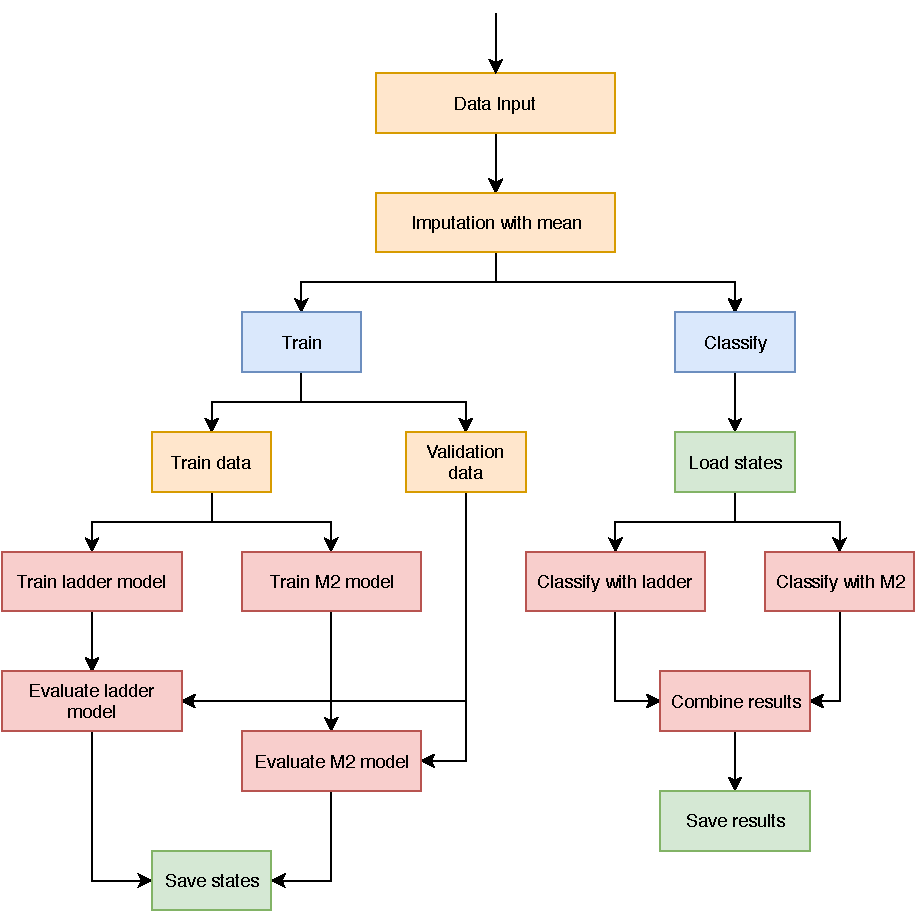
\includegraphics[scale=1]{figs/tool.pdf}
  \caption{Pipeline of the tool}
  \label{fig:saliency}
\end{figure}

\chapter{Conclusion}

\textit{This dissertation has discussed the researching, implementation and evaluation of several semi-supervised models for use with genomic
data. It has also discussed techniques for processing data and improving model performance, and has used the lessons learned from 
this to construct a simple command line tool.}

\section{Success Criteria}

All the major success criteria of the project have been achieved. 

The implementations of the models performed as well as their original paper implementations on the MNIST dataset, showing that they were 
implemented correctly. All the models are now available online at https://github.com/Clondon98/Semi-Supervised\_Models, and include the 
best performing PyTorch implementation of the semi-supervised VAE and ladder that I was able to find online. This repository also allows 
the models to be easily used on different datasets, while other implementations are restricted to MNIST. 

The M2 and ladder model also succeeded in achieving statistically significant performance improvements over the fully supervised model on 
gene expression data, and an average of both of the models achieved even higher performance. This led to the development of a 
command line tool that can be trained and used for classification very simply, with no need for knowledge of machine learning techniques.

I also managed to implement an extension that calculated the saliency of inputs to the network, and while I ran out of time to include it 
in the tool, the results on MNIST showed that it was locating important features for the classification of the characters.

\section{Further Work}

Some areas of the project that could be explored further include:
\begin{itemize}
    \item Using VAEs to generate additional unlabelled datapoints and adding these to the dataset to see if they improve performance.
    \item Using a semi-supervised VAE to generate additional labelled datapoints and seeing if these help improve supervised learning 
          performance.
    \item Discovering the most important genes for phenotypes using saliency and comparing those to highly important genes found through
          other methods.  
\end{itemize}

\section{Final remarks}

I hope that the models used in this project can be refined further to find real use in the fields of medicine and biology. The models and tool
developed in this project are all freely available online and will hopefully be of use to future researchers interested in semi-supervised
learning.

\addcontentsline{toc}{chapter}{Bibliography}
\printbibliography

\appendix

\chapter{Backpropagation} \label{backprop}

Backpropagation is the flow of information from the outputs of the network back through the network. Once the cost function has been computed
finding the gradient of the loss with respect to each trainable parameter shows which direction the parameter can be shifted to decrease 
the loss function.. This derivation of the backpropagation algorithm is based on that found in \textit{Artificial intelligence I}~\cite{Art_Int}.
In the derivations below:
\begin{itemize}
  \item $J(\vec{\theta})_k$ is the cost function for the $kth$ sample in the training set
  \item $w_{i \to j}$ is the weight between node $i$ and node $j$
  \item $a_j$ is the value computed by the node $j$ pre-activation ($\sum_{k} w_{k \to j} z_k$)
  \item $z_j$ and $y_j$ are the values post-activation ($\sigma(a_j)$), for non-output and output nodes respectively
\end{itemize}

The value to be calculated for each weight (per sample) is $\frac{\partial J(\vec{\theta})_k}{\partial w_{i \to j}}$. To do this we use the chain rule
of differentiation:
\begin{align}
  \frac{\partial J(\vec{\theta})_k}{\partial w_{i \to j}} & = \frac{\partial J(\vec{\theta})_k}{\partial a_j} \frac{\partial a_j}{\partial w_{i \to j}} \\
  & = \frac{\partial J(\vec{\theta})_k}{\partial a_j} z_i
\end{align}

Then for weights connected to the output nodes:
\begin{align}
  \frac{\partial J(\vec{\theta})_k}{\partial w_{i \to j}} & = \frac{\partial J(\vec{\theta})_k}{\partial a_j} z_i \\
  & = \frac{\partial J(\vec{\theta})_k}{\partial y_j} \frac{\partial y_j}{\partial a_j} z_i
\end{align}

If our loss function is differentiable with respect to $y_j$, and $y_j$ is differetiable with respect to $a_j$ then we can calculate this.  
For backpropagation to work all our loss and activation functions must have this property. Thankfully all the loss and activation functions 
shown in this dissertation do have that property and so work correctly with backpropagation.

Once the gradients are computed for the weights in the output layer it is possible to calculate them for the next layer, and then the
layer after that, etc., as the errors are backpropagated through the network. The computation for the hidden layers is slightly more 
complicated:
\begin{align}
  \frac{\partial J(\vec{\theta})_k}{\partial w_{i \to j}} & = \frac{\partial J(\vec{\theta})_k}{\partial a_j} z_i \\
  & = \left( \sum_{k \in K} \frac{\partial J(\vec{\theta})_k}{\partial a_k} \frac{\partial a_k}{\partial a_j} \right) z_i
\end{align}
\begin{center}
  \textit{where K is the set of all nodes $j$ is connected to in the next layer}
\end{center}

By definition:
\begin{align}
  \frac{\partial a_k}{\partial a_j} & = \frac{\partial}{\partial a_j} \left( \sum_{i} w_{i \to k} z_i \right) \\
  & = \frac{\partial}{\partial a_j} \left( \sum_{i} w_{i \to k} \sigma(a_i) \right) \\
  & = w_{j \to k} \sigma'(a_j)
\end{align}

Therefore, for hidden layers:
\begin{align}
  \frac{\partial J(\vec{\theta})_k}{\partial w_{i \to j}} & = \left( \sum_{k \in K} w_{j \to k} \frac{\partial J(\vec{\theta})_k}{\partial a_k} \right) \sigma'(a_j) z_i
\end{align}

As the errors are moving backward through the network, and all nodes $k$ are in the layer after $j$, $\frac{\partial J(\vec{\theta})_k}{\partial a_k}$
has already been computed and so this gradient can be calculated.

\chapter{Derivation of VAE loss} \label{vae_loss}

\begin{align}
  \log p(x) & = \log \int p(x|z)p(z) dz &\text{Law of total probability}\\
  & = \log \int p(x|z)p(z) \frac{q(z|x)}{q(z|x)} dz\\
  & = \log\left(\mathbb{E}_q \left[\frac{p(x|z)p(z)}{q(z|x)}\right]\right) \\
  & \geq \mathbb{E}_q \left[\log\frac{p(x|z)p(z)}{q(z|x)}\right] &\text{Jensen's inequality}\\
  & = \mathbb{E}_q \left[\log p(x|z) + \log\frac{p(z)}{q(z|x)}\right] \\
  & = \mathbb{E}_q [\log p(x|z)] - D_{KL}(q(z|x)||p(z))
\end{align}

\chapter{The reparameterization trick} \label{reparam}

It is not possible to backpropagate the reconstruction loss of a varitaional autoencoder through the random sampling in the latent dimension, because the drawing of
the samples is not differentiable with respect to $\vec{\mu}$ and $\vec{\sigma}$. Previously this was solved using a Monte Carlo gradient estimator, but these have 
extremely high variance and are impractical.Instead the reparameterization trick allows the Gaussian sample to be reparameterized as:
\begin{align}
  \vec{z_{i}} = \vec{\mu} + \vec{\sigma}\vec{\epsilon}
\end{align}

$\vec{\epsilon}$ is a vector of samples from the standard normal distribution $\mathcal{N}(0, 1)$. The sampling operation is now differentiable
with respect to $\vec{\mu}$ and $\vec{\sigma}$ and therefore is differentiable with respect to $\vec{\theta}$, the trainable parameters of the encoder. As the
gradients can be backpropagated through the network it is possible to train the VAE using gradient descent.

\chapter{Derivation of semi-supervised VAE loss} \label{ssvae_loss}

For labelled data the model should maximise evidence $\log p(\vec{x}, y)$:
\begingroup
\allowdisplaybreaks
\begin{align*}
  \log p(x, y) & = \log \int p(x, y, z) dz \\
  & = \log \int p(x|y, z)p(y)p(z) dz \qquad \text{Independence of $z$ and $y$}\\
  & = \log \int p(x|y, z)p(y)p(z) \frac{q(z|x, y)}{q(z|x, y)} dz\\
  & = \log\left(\mathbb{E}_q \left[\frac{p(x|y, z)p(y)p(z)}{q(z|x, y)}\right]\right) \\
  & \geq \mathbb{E}_q \left[\log\frac{p(x|y, z)p(y)p(z)}{q(z|x, y)}\right] \\
  & = \mathbb{E}_q \left[\log p(x|y, z) + \log p(y) + \log\frac{p(z)}{q(z|x, y)}\right] \\
  & = \mathbb{E}_q [\log p(x|y, z) + \log p(y)] - D_{KL}(q(z|x, y)||p(z)) \\
  & = -\mathcal{L}(x, y)
\end{align*}
\endgroup

For unlabelled data the model should maximise $\log p(\vec{x})$:
\begingroup
\allowdisplaybreaks
\begin{align*}
  \log p(x) & = \log \sum_{y} \int p(x, y, z) dz \\
  & = \log \sum_{y} \int p(x, y, z) \frac{q(z, y|x)}{q(z, y|x)} dz\\
  & = \log \sum_{y} \int p(x, y, z) \frac{q(z|x, y)q(y|x)}{q(z|x, y)q(y|x)} dz\\
  & \geq \sum_{y} q(y|x) \int q(z|x, y) \log\frac{p(x, y, z)}{q(z|x, y)q(y|x)} dz \qquad \text{Jensen's inequality}\\
  & = \sum_{y} q(y|x) \int q(z|x, y) \log\frac{p(x, y, z)}{q(z|x, y)} dz - \sum_{y} q(y|x) \log q(y|x) \int q(z|x, y) dz\\
  & = \sum_{y} q(y|x)(-\mathcal{L}(x, y)) + \mathcal{H}(q(y|x)) \\
  & = -\mathcal{U}(x, y)
\end{align*}
\endgroup

\chapter{Confusion matrices} \label{confusion}

\begin{figure}[H]
  \centering
  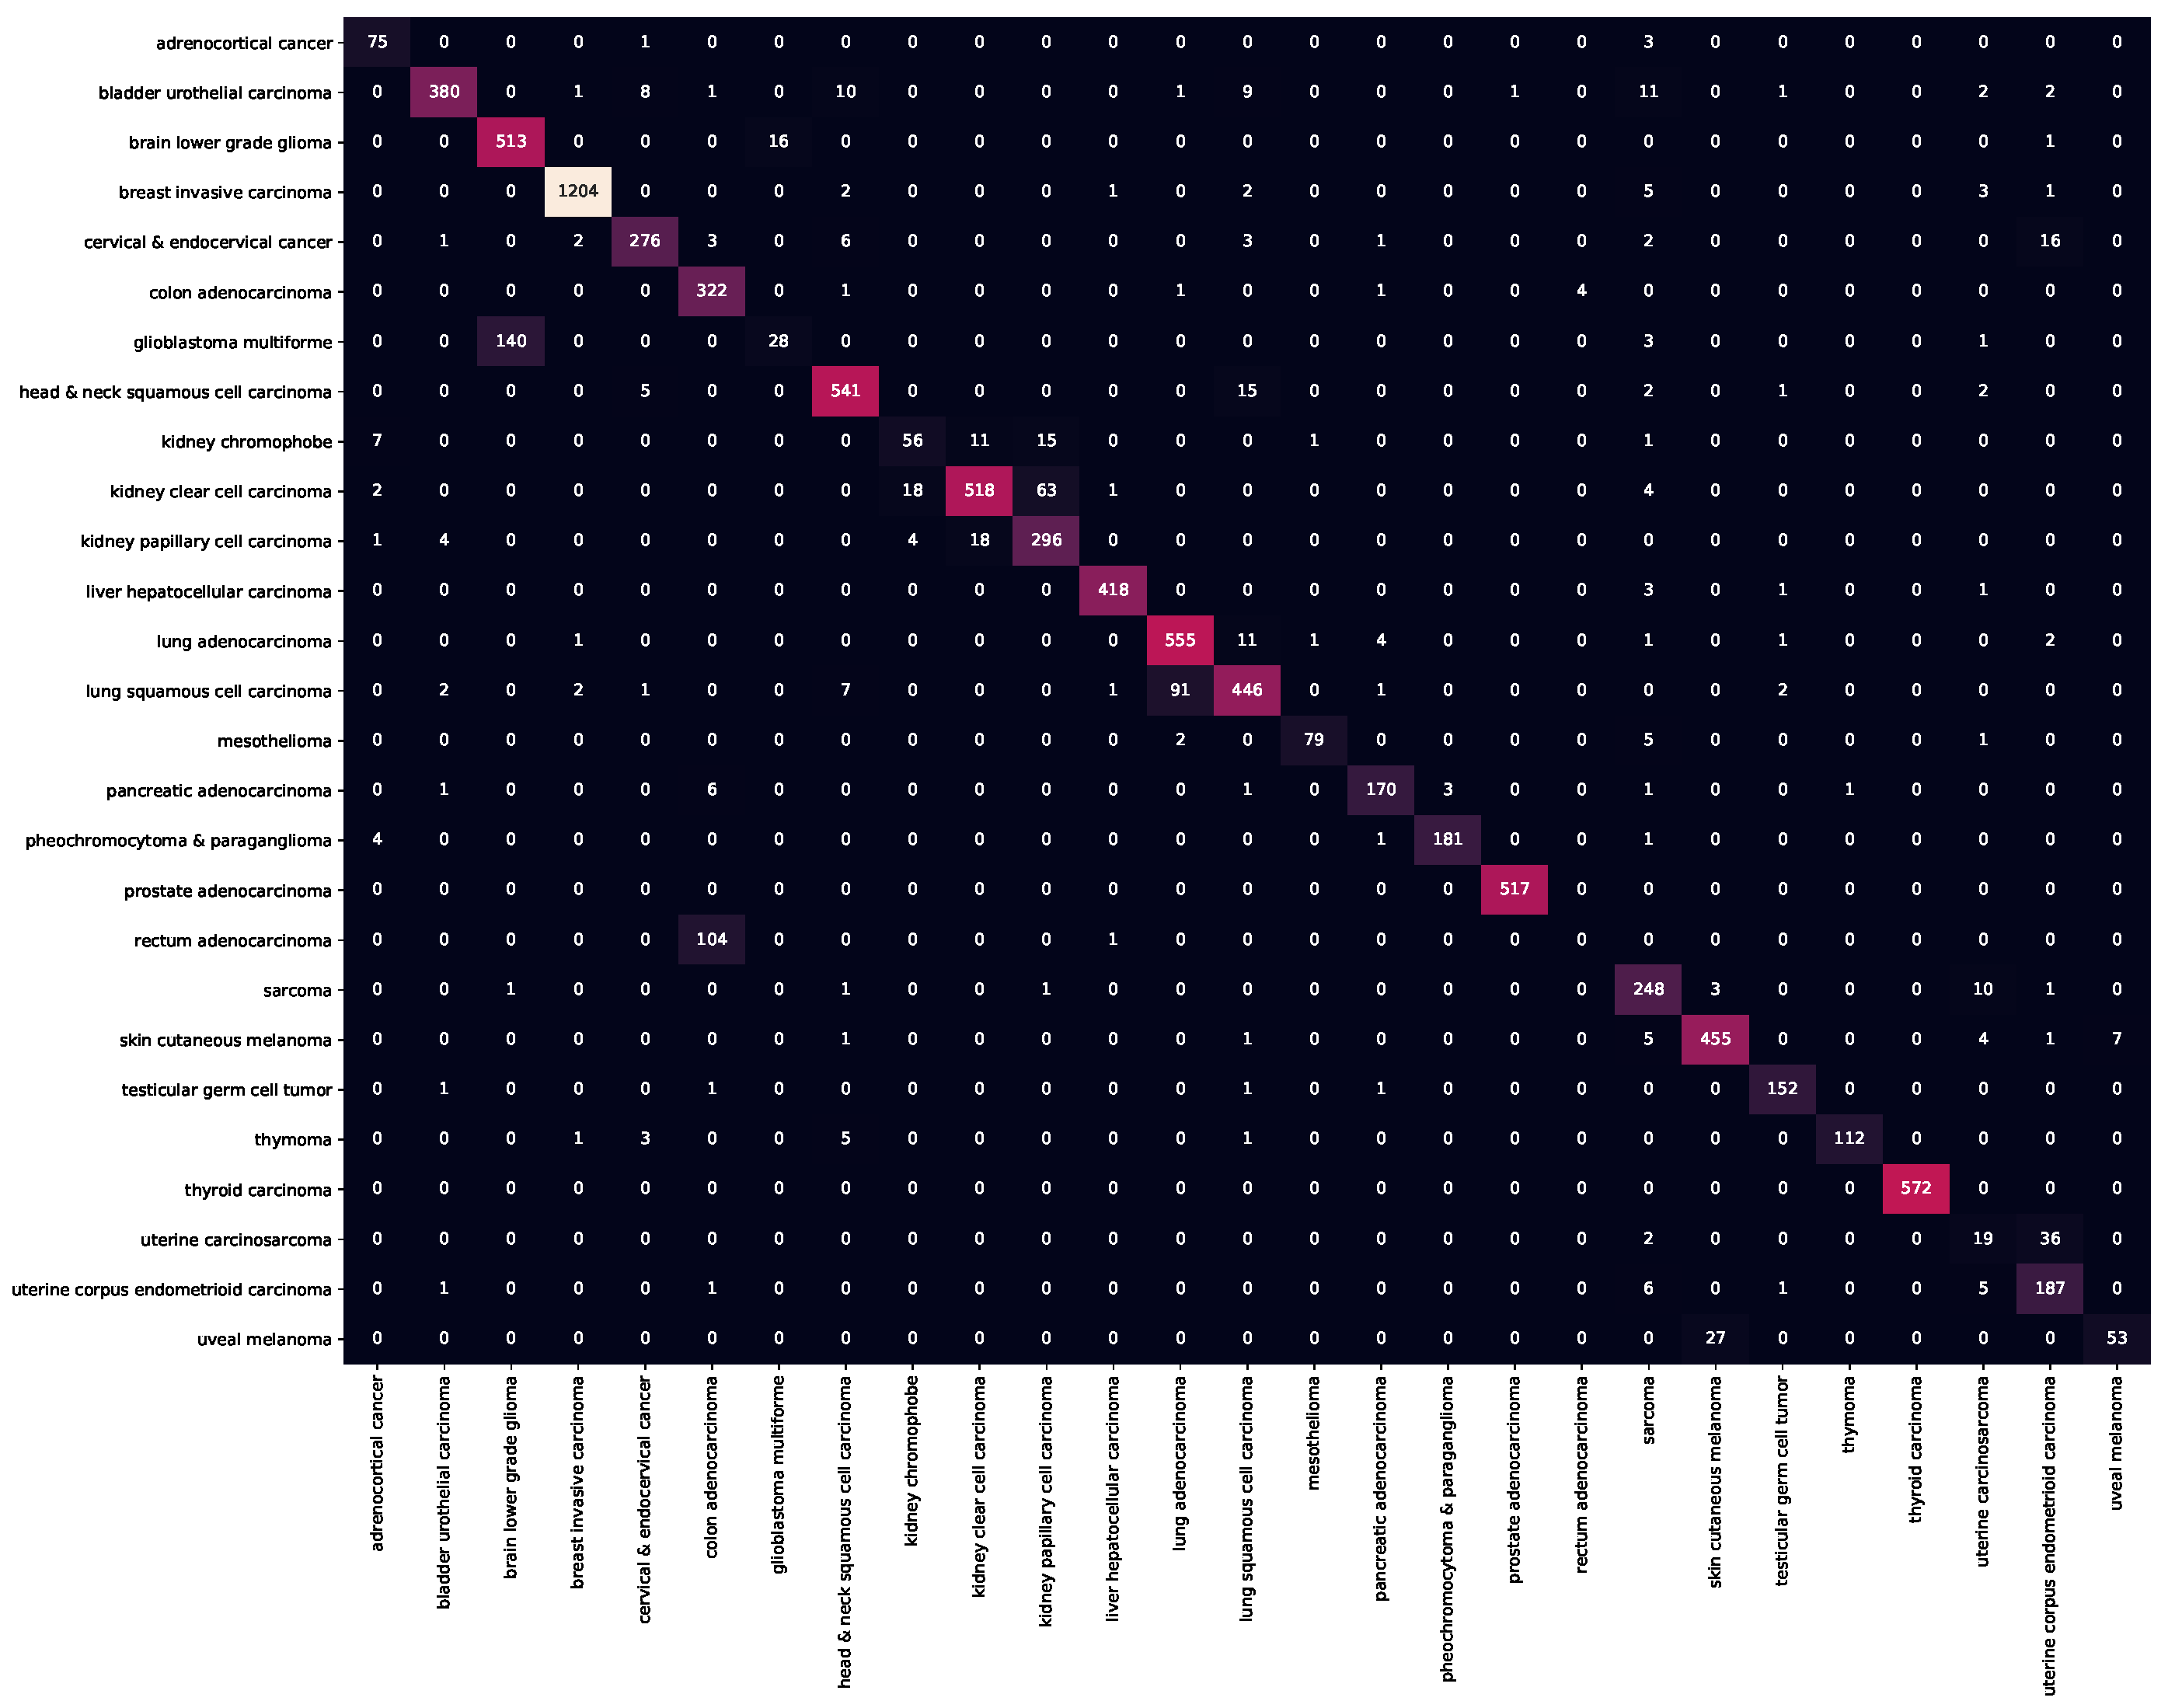
\includegraphics[scale=0.4, angle=90]{figs/m2_tcga_minmax_m2_100.pdf}
  \caption{Confusion matrix for M2 model with 100 labels}
\end{figure}

\begin{figure}[H]
  \centering
  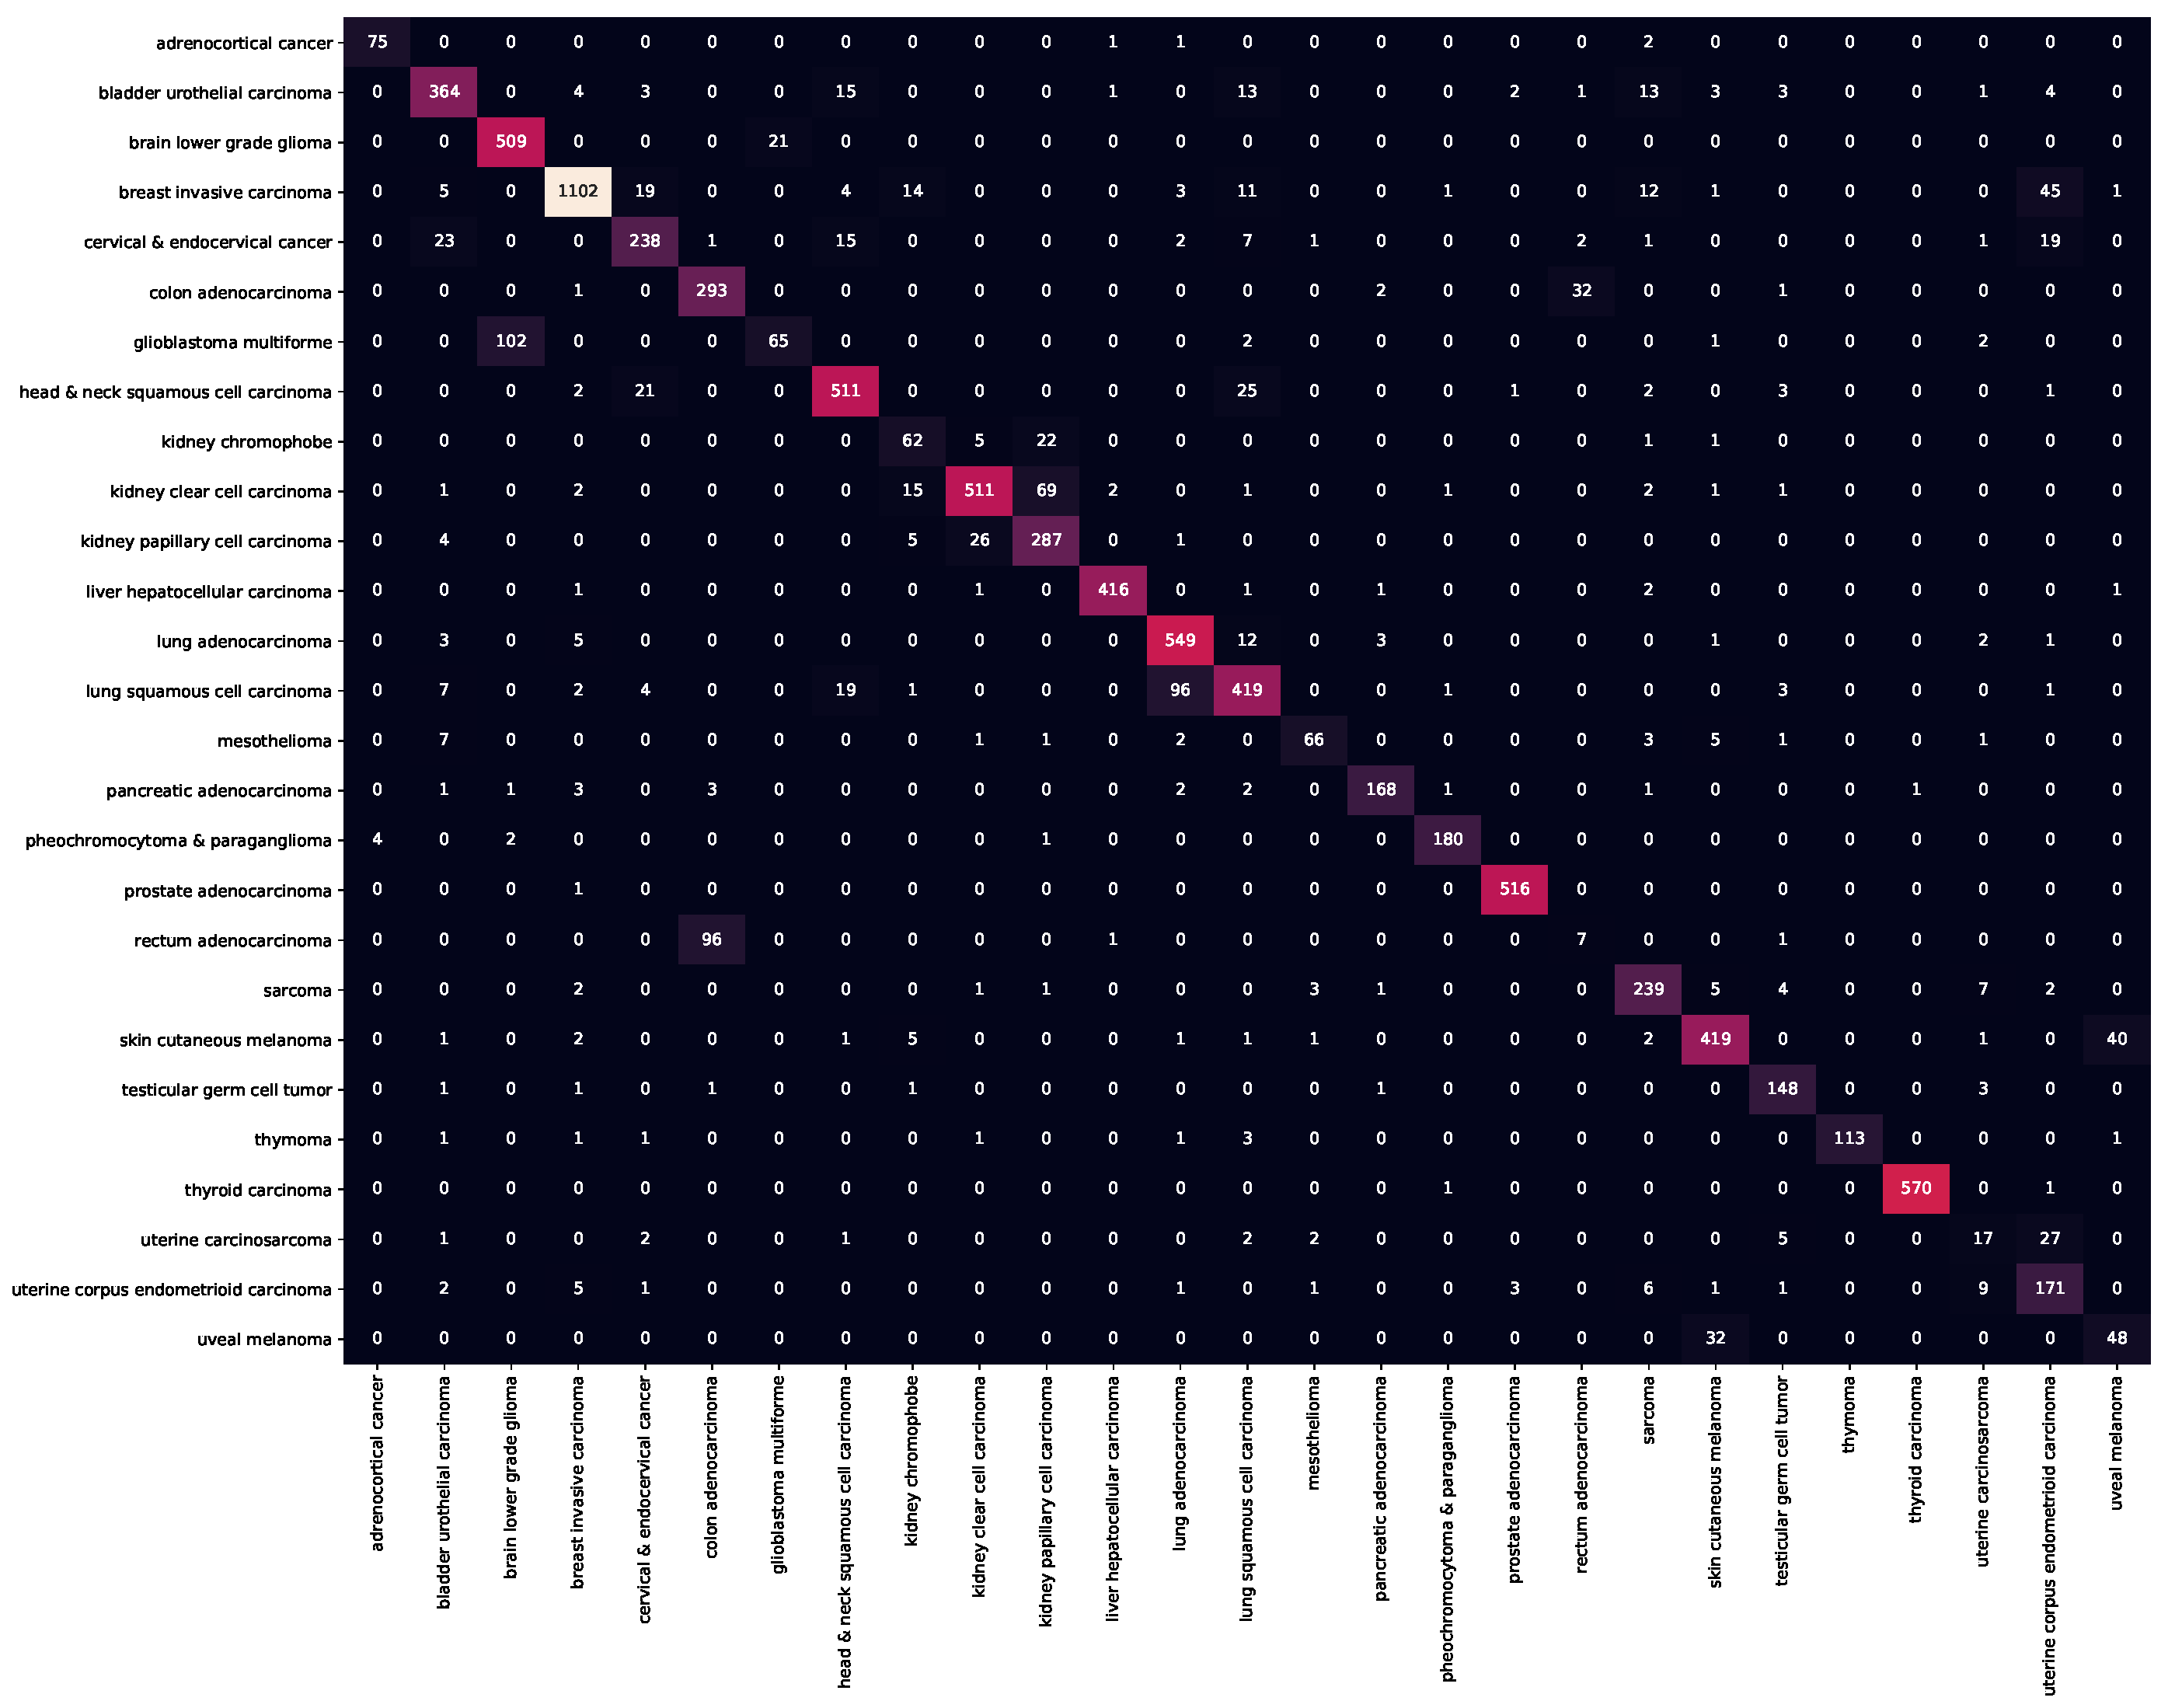
\includegraphics[scale=0.4, angle=90]{figs/ladder_tcga_standard_100.pdf}
  \caption{Confusion matrix for the ladder model with 100 labels}
\end{figure}

\chapter{Project Proposal} \label{proposal}
% Note: this file can be compiled on its own, but is also included by
% diss.tex (using the docmute.sty package to ignore the preamble)
\documentclass[12pt,a4paper,twoside,openany]{article}
\usepackage[pdfborder={0 0 0}]{hyperref}
\usepackage[margin=25mm]{geometry}
\usepackage{graphicx}
\usepackage{parskip}

\begin{document}

\begin{center}
\Large
Computer Science Tripos -- Part II -- Project Proposal\\[4mm]
\LARGE
A tool for phenotype prediction from cell genotype

\large
C.~London, Trinity College

Originator: Prof P.~Li\'o \& H.~Andres~Terre

19 October 2018
\end{center}

\vspace{5mm}

\textbf{Project Supervisor:} Prof P.~Li\'o \& H.~Andres~Terre

\textbf{Director of Studies:} Prof F.~Stajano

\textbf{Project Overseers:} Prof J.~Daugman  \& Dr A.~Madhavapeddy

% Main document

\section*{Introduction}

Phenotype prediction from cell genotype is an important problem in the field of bioinformatics, with usages in agriculture (for selecting crops with highest yield potential), medicine (for predicting likelihood of diseases/mutations), research, and many other fields. With the decreasing cost of genome sequencing this is becoming far more feasible for use in both research and the private sector.

Deep learning techniques provide an opportunity for generating high accuracy predictions of the phenotype from the genotype and as such much research in this area uses techniques such as autoencoders and neural networks to attempt to do this. However, much of the state of the art research is focused on generating predictions for only one type of cell, and so the network is structured specifically towards this cell. This is then not generalisable and not useful in other scenarios.

This project aims to build a tool that will provide these high accuracy predictions and is generalisable to data from different cells. By providing genotype data tagged with the observed phenotype for training, a user should then be able to use this tool to predict the required phenotype.

\section*{Starting point}

\subsection*{Prior Research}

This project is based on similar state of the art work done in papers on DeepGS\cite{DeepGS} (genomic selection) and DeepMetabolism\cite{DeepMetabolism}.

DeepGS was used to predict several phenotypes (grain length, grain hardness, plant height and more for wheat) when given genomic markers, and is now available as an R library. However the method  uses convolution and sampling to reduce data dimensionality, whereas the DeepMetabolism uses unsupervised pre-training in the form of an autoencoder to speed the supervised learning up. I believe that this is the better way to do it, and prescribes a less rigid structure on the model.

DeepMetabolism was used to predict three phenotypes of \textit{Escherichia Coli} and uses unsupervised pre-training with an autoencoder. However the autoencoder is used for denoising purposes, and the output, a cleaned version of the input data, is used for predictio instead of using the latent representation. The autoencoder is also structured specifically to correspond to the genome and proteins of \textit{E. Coli} and so the re-usability is limited.

\subsection*{Libraries and codebase}

The code for the learning will be written in Python, because Python has excellent support for advanced deep learning libraries. I have written machine learning code in Python before using Scikit-learn, but for this project I will use either Tensorflow or PyTorch as these libraries provide much better support for deep learning applications, as well as allowing for data parallelism and therefore large speed-ups when running on a GPU.

\section*{Resources required}

For this project I shall mainly use my own laptop, a 2014 Macbook Pro with a dual core Intel i5, 8GB of RAM and 128GB of flash storage. Source code for the project will be kept in a Git repository that will be synced with a repository on Github. The \LaTeX\\ source will be stored on my machine, and backed up to both overleaf.com and Google Drive. The entire content of my laptop will be frequently backed up to an external 500GB HDD.

The training of the model will be done using GPUs that can be provided by the Computer Lab, with confirmation from Professor Li\'o.

Data for training and testing the model will be both artificially generated as part of the project, and provided by the Plant Sciences department.

\section*{Work to be done}

\subsection*{Reading and further research}

\begin{itemize}
    \item Re-read papers on DeepGS and DeepMetabolism looking for particular insight into the exact models used to see ways they could be improved.
    
    \item Deep learning to model the hierarchical structure of the cell[3] - this is less relevant to the project as it involves a neural network that is pre-structured by hand, but still involves genotype-phenotype prediction and so may contain useful insights.
    
    \item Principles of gene manipulation and genomics\cite{Genomics} Chapters 16 to 20 - a book about genome analysis, involving genomic and transcriptomic data. This is necessary because I have never worked on a project with large scale genome analysis before.
    
    \item Reducing the dimensionality of data using neural networks\cite{Encoders} - information on reducing the dimensionality of data using autoencoders.
    
    \item Sparse autoencoders (lecture notes by Andrew Ng) - more information about using autoencoders to learn the most important features of data unsupervised.
    
    \item Meetings with Prof. Haseloff - Prof. Haseloff is a member of the plant sciences department here at the university and has experience working with the Computer Lab on other bioinformatics projects. He should be able to provide real data to use in training, as well as insight into what the synthetic data should look like.
    
\end{itemize}

\subsection*{The model}

The model for predicting the phenotype will be split into unsupervised and supervised portions.

The unsupervised portion is used to for dimesionality reduction of data, and is effectively a sort of pre-training for the model. Genomic data can be very large depending on the cell and so reducing the dimensionality to only the most important features should significantly speed the model up, and should hopefully provide greater prediction accuracy. This pre-training is likely to involve passing the genomic data into an autoencoder. An autoencoder is made up of two parts, an encoder and a decoder. The encoder includes the input layer and some hidden layers culminating in a final layer that has fewer nodes than the input layer. This layer is the latent representation of the input data. The decoder then attempts to reconstruct the input data from this representation, and backpropagation is performed to get the reconstruction as close as possible to the original. This latent representation should then be the features of the data that are most important for accurate reconstruction, and is therefore a reduced dimensionality representation of the data.

The supervised portion of the model will take the form of a neural network that takes in this latent representation as input and outputs the predicted phenotype. Backpropagation is performed to train the network to accurately predict the phenotype.

An important feature of the model should be the ability to work with different sized inputs and outputs. For the model to be generalisable to different cells, it will have to be able to take variable sized genome inputs, as the length of a genome sequence varies greatly between organisms. The output size will also not always be constant as the phenotype can take many forms - sometimes it might simply be a number e.g. if the studied phenotype is plant height, whereas other times it could be a class, or, as written in the extensions below, a photograph.

\paragraph{Testing.}

Testing the model will first be done with synthetic data, to ensure that it is working as it should i.e. recognising patterns and correctly identifying the most important features in the data, and the phenotype that should be associated with a given latent representation. The generation of this synthetic data will form an early part of this project, and will be done with input from Prof. Haseloff as he has significant experience with biological data.  

Once this is completed the model will then be trained and tested on real world data to verify its accuracy and usefulness as a real world prediction tool.

\subsection*{The tool}

This project should lead to a tool that can be used to predict phenotype without requiring users to know much about the underlying machine learning. To that end the tool should provide a basic front-end where users can add a file with training data, and, once training has completed, provide data that they want predictions for. The difficulty here is dealing with the different phenotypes a user might want, and having a model that can handle very different output requirements.

\section*{Success criteria}

Evaluation of the success of the project will be based upon the following criteria:

\begin{itemize}
    \item Better prediction accuracy than supervised training alone on a synthetic dataset (generated as part of the project) - compare the predicted phenotype with the synthetic phenotype generated for a particular pattern in the synthetic genotype data.
    \item Better prediction accuracy than supervised training alone on real world genotype and phenotype data.
    \item Producing a tool with a front-end that takes a file-path and trains the model based on the data within the file.
\end{itemize}

Prediction accuracy can be compared using a statistical significance test. The models will be trained on the same dataset and then tested on data that was not part of the training set. With synthetic data it is easy to generate data that was not part of the training set. With real world data if there is not enough for a separate training set and test set k-fold cross-validation can be performed.

\section*{Possible extensions}

If the main result is achieved and time is left some possible extensions are:

\begin{itemize}
    \item Use images of a cell/plant/etc. as the phenotype for training, and generate images as predictions. This would involve using other deep learning techniques to generate the images, likely generative adversarial networks.
    
    \item Measuring the importance of inputs to the output. Neural networks are often considered to be a sort of black box where input goes in and a result comes out. It is possible however to use some techniques to discover the importance of the input to the result. This can then be used to pinpoint which genes were most responsible for a certain phenotype. However, results can be misleading and the accuracy is not always good.
    
    \item Autoencoder structure based upon cell structure. Some well-studied organisms have extensive prior knowledge about gene interactions available in resources such as the Gene Ontology which would enabling structuring the autoencoder such that it partially mimics the cell. This should speed up training and could increase prediction accuracy. It would not be available for all cells, but if a user was using a well-studied cell the option to use a structured autoencoder would be useful.
\end{itemize}


\section*{Timetable}

Planned starting date is 20/10/2018.

\begin{enumerate}

\item \textbf{20/10/2018 -- 3/11/2018 } 

Perform the reading and research as stated in the "Work to be done" section. Install Tensorflow and PyTorch and decide which to use by doing small example learning tasks.

\item \textbf{4/11/2018 -- 18/11/2018} 

Write Python code to generate synthetic data for training. Begin building unsupervised model. Begin writing Introduction and Preparation chapters of dissertation.

\item \textbf{19/11/2018 -- 3/12/2018} 

Train and tune unsupervised model on synthetic data. Ensure that features expected to be important have large impact. Begin building supervised model. Begin writing Implementation chapter of dissertation.

\item \textbf{Michaelmas vacation} 

Do supervised training using output from the unsupervised model as input to the network. Make sure model is generalisable to different sized inputs and outputs corresponding to different cells and phenotypes.

\textbf{Milestones:}
\begin{itemize}
    \item Have a working prediction model trained on the synthetic data.
    \item Have finished writing dissertation Introduction and Preparation chapters.
\end{itemize}

\item \textbf{15/01/2019 -- 29/01/2019} 

Write progress report. Compare accuracy of model against a simple supervised model on artificial data to ensure model has better accuracy. Begin writing Evaluation chapter of dissertation.

\item \textbf{30/01/19 -- 13/02/19} 

Train model on real data and compare prediction accuracy with only supervised network.

\textbf{Milestones:}
\begin{itemize}
    \item Progress report submitted on 01/02/19.
\end{itemize}

\item \textbf{14/02/19 -- 28/02/19} 

Build a front-end that allows a user to pass a file of training data and create a model. Begin Extension 1: using images as phenotype.

\textbf{Milestones:}
\begin{itemize}
    \item Have a working tool allowing users to provide their own data for training.
    \item Have completed the Implementation chapter of the dissertation.
\end{itemize}

\item \textbf{01/03/19 -- 15/03/19} 

Extension 2: Pinpointing genes that have the greatest effect on phenotype.
Ensure full evaluation of all success criteria. Begin writing dissertation Evaluation chapter.

\item \textbf{Easter vacation}  

Writing dissertation and finishing any ongoing extensions. Extension 3 if time allows.

\item \textbf{23/04/19 -- 7/5/19} 

Proof reading, performing any final changes recommended by supervisor, preparing for submission in order to focus on exams.

\textbf{Milestone:} Have a completed and checked dissertation.

\end{enumerate}

\begin{thebibliography}{}
\bibitem{DeepGS} 
Ma W. \& Qiu Z. (2017) \textit{DeepGS: Predicting phenotypes from genotypes using Deep Learning}
\bibitem{DeepMetabolism}
Guo W., Xu Y. \& Feng X. (2017) \textit{DeepMetabolism: A Deep Learning System to Predict Phenotype from Genome Sequencing}
\bibitem{CellStructure}
Ma J., Yu M., Fong S., \& Ideker T. (2018) \textit{Using deep learning to model the hierarchical structure and function of a cell}
\bibitem{Genomics}
Primrose S. \& Twyman R. (2006) \textit{Principles of Gene Manipulation and Genomics}
\bibitem{Encoders}
Hinton G. \& Salakhutdinov R. (2006) \textit{Reducing the Dimensionality of Data with Neural Networks}

\end{thebibliography}

\end{document}

\end{document}
